\section{Satellite imagery and ground truth data}\label{app:satellite_imagery}

\subsection{Study region covering}

We obtained a total of 60 Planetscope satellite images covering the
coast of the Balearic Islands for the years 2020 to 2023. From those, the 20
images covering the island of Mallorca for years 2020-2022 were used to conform
the training
dataset, while the images from the other islands for the years 2020-2022 were
included in the
out-of-sample test set (\cref{fig:images-dataset}). The resting images from the
whole region in the year 2023 were lft as final test. The metadata of the
satellite images used in the study is shown in
\cref{tab:metadata_satellite_images}.

\begin{figure}[H]
    \centering
    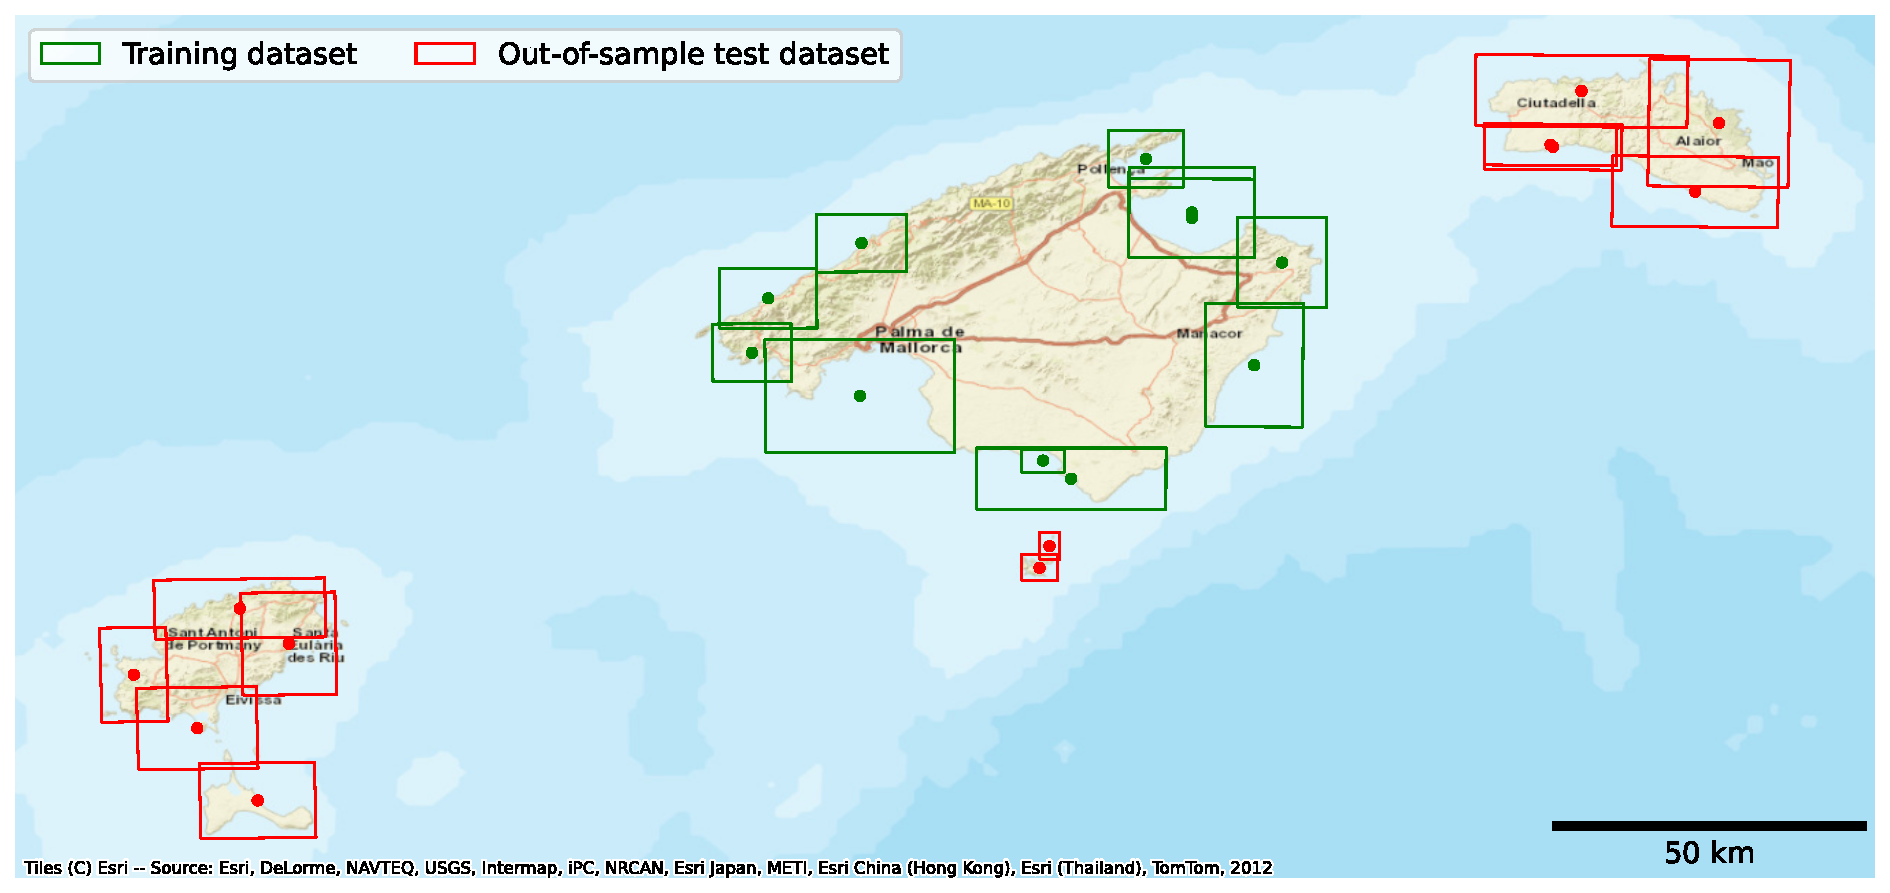
\includegraphics[width=\textwidth]{Figures/Images_used.pdf}
    \caption{Coverage of the training and out-of-sample test datasets in
        the Balearic Islands. Each image was obtained for different years
        from 2020 to 2023, depending on the availability.}
    \label{fig:images-dataset}
\end{figure}

Here we must emphasize that we refer to this test set as
``out-of-sample'' because the images conforming the set are relatively distant
to the ones in the training set. Furthermore, the sub-classes conforming the 4
major ecological classes are not exactly the same in each island (see below).
This, in principle, hinders the robustness and generalization ability of deep
learning models. Perhaps this is one of the reasons for which a general and
robust model for habitat mapping in the Mediterranean Sea has been hitherto
lacking. Thus, with this strict separation of training and out-of-sample test
set we aim to comprehensively study the robustness and generalization power of
our deep learning models.

Because we will finally train our model with all available data (from all
regions), the images from 2023 will conform the final test set, to ensure the
robustness of the model to changes in environmental conditions at the moment of
image acquisition and image metadata.

% \usepackage{tabularray}
\begin{longtblr}[
    caption = {Metadata of the satellite images used in the study.},
    label = {tab:metadata_satellite_images},
    ]{
    width = \linewidth,
    colspec = {Q[417]Q[200]Q[154]Q[167]},
    row{1} = {c},
    cell{2}{2} = {c},
    cell{2}{3} = {c},
    cell{2}{4} = {c},
    cell{3}{2} = {c},
    cell{3}{3} = {c},
    cell{3}{4} = {c},
    cell{4}{2} = {c},
    cell{4}{3} = {c},
    cell{4}{4} = {c},
    cell{5}{2} = {c},
    cell{5}{3} = {c},
    cell{5}{4} = {c},
    cell{6}{2} = {c},
    cell{6}{3} = {c},
    cell{6}{4} = {c},
    cell{7}{2} = {c},
    cell{7}{3} = {c},
    cell{7}{4} = {c},
    cell{8}{2} = {c},
    cell{8}{3} = {c},
    cell{8}{4} = {c},
    cell{9}{2} = {c},
    cell{9}{3} = {c},
    cell{9}{4} = {c},
    cell{10}{2} = {c},
    cell{10}{3} = {c},
    cell{10}{4} = {c},
    cell{11}{2} = {c},
    cell{11}{3} = {c},
    cell{11}{4} = {c},
    cell{12}{2} = {c},
    cell{12}{3} = {c},
    cell{12}{4} = {c},
    cell{13}{2} = {c},
    cell{13}{3} = {c},
    cell{13}{4} = {c},
    cell{14}{2} = {c},
    cell{14}{3} = {c},
    cell{14}{4} = {c},
    cell{15}{2} = {c},
    cell{15}{3} = {c},
    cell{15}{4} = {c},
    cell{16}{2} = {c},
    cell{16}{3} = {c},
    cell{16}{4} = {c},
    cell{17}{2} = {c},
    cell{17}{3} = {c},
    cell{17}{4} = {c},
    cell{18}{2} = {c},
    cell{18}{3} = {c},
    cell{18}{4} = {c},
    cell{19}{2} = {c},
    cell{19}{3} = {c},
    cell{19}{4} = {c},
    cell{20}{2} = {c},
    cell{20}{3} = {c},
    cell{20}{4} = {c},
    cell{21}{2} = {c},
    cell{21}{3} = {c},
    cell{21}{4} = {c},
    cell{22}{2} = {c},
    cell{22}{3} = {c},
    cell{22}{4} = {c},
    cell{23}{2} = {c},
    cell{23}{3} = {c},
    cell{23}{4} = {c},
    cell{24}{2} = {c},
    cell{24}{3} = {c},
    cell{24}{4} = {c},
    cell{25}{2} = {c},
    cell{25}{3} = {c},
    cell{25}{4} = {c},
    cell{26}{2} = {c},
    cell{26}{3} = {c},
    cell{26}{4} = {c},
    cell{27}{2} = {c},
    cell{27}{3} = {c},
    cell{27}{4} = {c},
    cell{28}{2} = {c},
    cell{28}{3} = {c},
    cell{28}{4} = {c},
    cell{29}{2} = {c},
    cell{29}{3} = {c},
    cell{29}{4} = {c},
    cell{30}{2} = {c},
    cell{30}{3} = {c},
    cell{30}{4} = {c},
    cell{31}{2} = {c},
    cell{31}{3} = {c},
    cell{31}{4} = {c},
    cell{32}{2} = {c},
    cell{32}{3} = {c},
    cell{32}{4} = {c},
    cell{33}{2} = {c},
    cell{33}{3} = {c},
    cell{33}{4} = {c},
    cell{34}{2} = {c},
    cell{34}{3} = {c},
    cell{34}{4} = {c},
    cell{35}{2} = {c},
    cell{35}{3} = {c},
    cell{35}{4} = {c},
    cell{36}{2} = {c},
    cell{36}{3} = {c},
    cell{36}{4} = {c},
    cell{37}{2} = {c},
    cell{37}{3} = {c},
    cell{37}{4} = {c},
    cell{38}{2} = {c},
    cell{38}{3} = {c},
    cell{38}{4} = {c},
    cell{39}{2} = {c},
    cell{39}{3} = {c},
    cell{39}{4} = {c},
    cell{40}{2} = {c},
    cell{40}{3} = {c},
    cell{40}{4} = {c},
    cell{41}{2} = {c},
    cell{41}{3} = {c},
    cell{41}{4} = {c},
    cell{42}{2} = {c},
    cell{42}{3} = {c},
    cell{42}{4} = {c},
    cell{43}{2} = {c},
    cell{43}{3} = {c},
    cell{43}{4} = {c},
    cell{44}{2} = {c},
    cell{44}{3} = {c},
    cell{44}{4} = {c},
    cell{45}{2} = {c},
    cell{45}{3} = {c},
    cell{45}{4} = {c},
    cell{46}{2} = {c},
    cell{46}{3} = {c},
    cell{46}{4} = {c},
    cell{47}{2} = {c},
    cell{47}{3} = {c},
    cell{47}{4} = {c},
    cell{48}{2} = {c},
    cell{48}{3} = {c},
    cell{48}{4} = {c},
    cell{49}{2} = {c},
    cell{49}{3} = {c},
    cell{49}{4} = {c},
    cell{50}{2} = {c},
    cell{50}{3} = {c},
    cell{50}{4} = {c},
    cell{51}{2} = {c},
    cell{51}{3} = {c},
    cell{51}{4} = {c},
    cell{52}{2} = {c},
    cell{52}{3} = {c},
    cell{52}{4} = {c},
    cell{53}{2} = {c},
    cell{53}{3} = {c},
    cell{53}{4} = {c},
    cell{54}{2} = {c},
    cell{54}{3} = {c},
    cell{54}{4} = {c},
    cell{55}{2} = {c},
    cell{55}{3} = {c},
    cell{55}{4} = {c},
    cell{56}{2} = {c},
    cell{56}{3} = {c},
    cell{56}{4} = {c},
    cell{57}{2} = {c},
    cell{57}{3} = {c},
    cell{57}{4} = {c},
    cell{58}{2} = {c},
    cell{58}{3} = {c},
    cell{58}{4} = {c},
    cell{59}{2} = {c},
    cell{59}{3} = {c},
    cell{59}{4} = {c},
    }
    \hline
    \textbf{Name}			 & \textbf{Satellite azimuth} &
    \textbf{Sun azimuth} & \textbf{Sun elevation} \\ \hline
    Formentera\_18\_july\_2021		 & 99.4 		      & 113.5
    & 57.3		      \\
    Formentera\_24\_july\_2022		 & 97.7 		      & 127.8
    & 63		      \\
    Formentera\_3\_august\_2023 	 & 110			      & 128.8
    & 60.5		      \\
    South\_Oeste\_Menorca\_29\_July\_2022  & 100.6		      & 116.1
    & 54.1		      \\
    South\_Oeste\_Menorca\_09\_July\_2021  & 182.4		      & 114.2
    & 58.1		      \\
    Sur\_Oeste\_Menorca\_9\_august\_2023	 & 101.5		      &
    121.5
    & 53.3		      \\
    Sur\_Ibiza\_20\_july\_2022		 & 101.1		      & 121.9
    & 61.4		      \\
    Sur\_Ibiza\_18\_july\_2021		 & 99.5 		      & 113.7
    & 57.3		      \\
    Sur\_Ibiza\_26\_august\_2023		 & 101.1		      &
    139.3
    & 55.5		      \\
    Es\_trenc\_25\_July\_2022		 & 270.7		      & 113.8
    & 54.6		      \\
    Es\_Trenc\_15\_july\_2023		 & 112.8		      & 112.6
    & 56.7		      \\
    Norte\_Menorca\_29\_July\_2021	 & 104.5		      & 136.3
    & 63		      \\
    Norte\_Menorca\_20\_July\_2022	 & 176.1		      & 118.6
    & 58.1		      \\
    Norte\_Menorca\_23\_june\_2023	 & 102			      & 123.6
    & 64.5		      \\
    Este\_Menorca\_19\_July\_2021	 & 271.4		      & 115.9
    & 56.7		      \\
    Este\_Menorca\_15\_July\_2022	 & 268			      & 113.3
    & 56.1		      \\
    Este\_Menorca\_23\_june\_2023	 & 266.2		      & 112.5
    & 58.8		      \\
    CalaPi\_CalaFiguera\_29\_july\_2021  & 100.9		      & 117.6
    & 55.7		      \\
    CalaPi\_CalaFiguera\_23\_july\_2022  & 101.8		      & 123.8
    & 60.8		      \\
    CalaPi\_CalaFiguera\_12\_july\_2023  & 155.9		      & 112.8
    & 57.5		      \\
    PortoColom\_CalaMillor\_27\_july\_2021 & 278			      &
    117.4
    & 55.9		      \\
    PortoColom\_CalaMillor\_22\_july\_2022 & 101.4		      & 123.9
    & 60.8		      \\
    PortoColom\_CalaMillor\_13\_july\_2023 & 101.7		      & 113.1
    & 57.5		      \\
    Sur\_Este\_menorca\_02\_July\_2021	 & 101.2		      & 130.5
    & 66.7		      \\
    Sur\_Este\_Menorca\_30\_July\_2022	 & 275.5		      & 116.4
    & 53.9		      \\
    Sur\_Este\_Menorca\_9\_august\_2023  & 273.9		      & 119.9
    & 52.4		      \\
    Palma\_7\_july\_2022			 & 102.1		      &
    120.9
    & 62.8		      \\
    Palma\_29\_june\_2023		 & 101.3		      & 123.1
    & 64.8		      \\
    Alcudia\_25\_July\_2022		 & 101			      & 125.1
    & 60.3		      \\
    Alcudia\_21\_May\_2020		 & 103.7		      & 119.7
    & 58.7		      \\
    Alcudia\_22\_July\_2021		 & 101.2		      & 133.1
    & 64.1		      \\
    Alcudia\_15\_july\_2023		 & 111.9		      & 113.2
    & 56.6		      \\
    Capdepera\_20\_july\_2021		 & 269.6		      & 115.5
    & 56.7		      \\
    Capdepera\_22\_july\_2022		 & 101.4		      & 123.9
    & 60.8		      \\
    Capdepera\_31\_july\_2023		 & 111.6		      & 116.2
    & 53.8		      \\
    Este\_Ibiza\_18\_july\_2021 	 & 99.6 		      & 113.8
    & 57.3		      \\
    Este\_Ibiza\_24\_july\_2022 	 & 98.1 		      & 128.6
    & 62.8		      \\
    Este\_Ibiza\_14\_july\_2023 	 & 277.5		      & 124
    & 63.3		      \\
    Pollença\_6\_July\_2021		 & 278.2		      & 113.9
    & 58.4		      \\
    Pollença\_23\_May\_2020		 & 277.1		      & 119.7
    & 58.8		      \\
    Pollença\_21\_July\_2022		 & 101.2		      & 124.2
    & 60.8		      \\
    Pollença\_27\_june\_2023		 & 106.9		      & 123.5
    & 64.4		      \\
    Oeste\_Ibiza\_18\_july\_2021		 & 101.6		      &
    113.8
    & 57.2		      \\
    Oeste\_Ibiza\_14\_july\_2022		 & 101.3		      &
    120.8
    & 62.3		      \\
    Oeste\_Ibiza\_19\_july\_2023		 & 277.3		      &
    112.6
    & 56.1		      \\
    Banyalbufar\_Soller\_23\_july\_2021  & 176.3		      & 116.8
    & 56.5		      \\
    Banyalbufar\_Soller\_17\_july\_2022  & 110.5		      & 123
    & 61.5		      \\
    Banyalbufar\_Soller\_12\_july\_2023  & 101.5		      & 124.5
    & 63.2		      \\
    Dragonera\_Banyalbufar\_29\_july\_2022 & 102.8		      & 120.4
    & 56.9		      \\
    Dragonera\_Banyalbufar\_10\_july\_2021 & 110.5		      & 113.7
    & 58.1		      \\
    Dragonera\_Banyalbufar\_16\_july\_2023 & 101.1		      & 125.8
    & 63.1		      \\
    Norte\_Ibiza\_18\_july\_2021		 & 101.6		      &
    113.8
    & 57.2		      \\
    Norte\_Ibiza\_18\_july\_2022		 & 277.9		      &
    112.7
    & 56.2		      \\
    Norte\_Ibiza\_27\_junio\_2023	 & 102			      & 110.9
    & 58.9		      \\
    South\_Cabrera\_23\_july\_2022	 & 101.8		      & 123.3
    & 60.9		      \\
    South\_Cabrera\_29\_june\_2023	 & 101.3		      & 110.7
    & 58.7		      \\
    North\_Cabrera\_19\_july\_2022	 & 101.7		      & 112
    & 55.5		      \\
    North\_Cabrera\_14\_july\_2023	 & 111.3		      & 124
    & 63.3 \\ \hline
\end{longtblr}

\subsection{Ground truth dataset composition}

The original seabed cartography contains a total of 28 different
classes, which were aggregated into 4 major ecological groups or habitat types
(\textit{Posidonia oceanica}, Other green plants, Brown algae \& rocks and
Sandy bottoms) based on feature similarity and ecological function
(\cref{tab:ecological_categories}). Although these habitat classes are present
in the whole Mediterranean Sea, the specific composition of underlying
sub-classes can vary among the different islands (e.g. one particular species
of algae might be present in only one island, such as \textit{Zostera noltii}).

\begin{table}
    \centering
    \caption{Ecological Categories and Subcategories in the ground truth
        habitat data.}
    \label{tab:ecological_categories}
    \resizebox{\columnwidth}{!}{%
        \begin{tabular}{|c|c|c|c|}
            \hline
            \textbf{Category}                 & \textbf{Subcategory}
                                              & \textbf{Area (km$^2$)}
                                              &

            \textbf{Presence zone}

            \\
            \hline
            \textbf{Posidonia oceanica}       & Posidonia oceanica
                                              & 538.61
                                              &
            Mallorca, Menorca, Ibiza, Formentera

            \\
                                              & Barrier reef of Posidonia
            oceanica
                                              & 0.49
                                              & Mallorca, Menorca
            \\
                                              & Posidonia oceanica on stone
            with
            sand                              & 20.33
                                              & Mallorca, Menorca
            \\
                                              & Mixed Posidonia oceanica with
            dead
            rhizome                           & 0.10
                                              & Ibiza
            \\
                                              & Meadows of Posidonia oceanica
            on
            dead mat (rhizome)                & 5.23
                                              &
            Mallorca, Menorca

            \\
            \hline
            \textbf{Other Green Plants}       & Algae photophilic on stone with
            Posidonia oceanica                & 6.63
                                              & Mallorca, Menorca
            \\
                                              & Caulerpa prolifera
                                              & 0.82
                                              & Mallorca, Menorca,
            Ibiza, Formentera
            \\
                                              & Meadows of phanerogams and
            green
            rhizomatous algae                 & 4.87
                                              &
            Mallorca, Menorca

            \\
                                              & Fine sands with Cymodocea
            nodosa
                                              & 1.95
                                              & Mallorca, Menorca,
            Ibiza, Formentera

            \\
                                              & Cymodocea nodosa
                                              & 1.86
                                              & Mallorca, Menorca,
            Ibiza, Formentera
            \\
                                              & Zostera noltii
                                              & 0.01
                                              & Menorca
            \\
                                              & Cymodocea nodosa and Zostera
            noltii                            & 0.04
                                              & Menorca
            \\
                                              & Mixed meadows of Cymodocea
            nodosa
            and Caulerpa prolifera            & 4.62
                                              &
            Mallorca, Menorca, Ibiza

            \\
                                              & Muddy bays with red algae
            (Alisidium corrallinum, Rytiphlaea
            tinctoria)                        & 0.01
                                              & Menorca
            \\
            \hline
            \textbf{Sandy Bottoms}            & Coarse sands
                                              & 250.19
                                              & Ibiza, Formentera
            \\
                                              & Soft or sedimentary substrate
                                              & 584.71
                                              & Mallorca, Menorca
            \\
                                              & Mud
                                              & 0.03
                                              & Ibiza
            \\
                                              & Fine sands
                                              & 74.36
                                              & Ibiza, Formentera
            \\
                                              & Muddy detrital bottom
                                              & 11.52
                                              & Ibiza
            \\
                                              & Leptometra phalangium fields in
            bathyal bottoms of platform edge
                                              & 208.85
                                              & Menorca
            \\
                                              & Bathyal bottoms of platform
            edge
            with Gryphus vitreus              & 91.93
                                              &
            Menorca

            \\
                                              & Medium sands
                                              & 42.41
                                              & Ibiza, Formentera
            \\
                                              & Muddy detrital bottoms
            infralittoral and circalittoral   & 589.81
                                              &
            Mallorca, Menorca, Formentera

            \\
            \hline
            \textbf{Brown Algae and Rocks}    & Rocky bottoms with photophilic
            algae and sands                   & 36.49
                                              & Mallorca, Menorca
            \\
                                              & Rocky bottoms dominated by
            sciafilic and hemisciafilic algae &
            21.17                             & Mallorca, Menorca, Ibiza,
            Formentera
            \\
                                              & Cliffs, walls, and rocky slopes
            of
            the deep sea                      & 13.96
                                              & Menorca
            \\
                                              & Rocky bottoms with photophilic
            algae                             & 14.35
                                              & Ibiza, Formentera
            \\
                                              & Rocky bottoms with photophilic
            algae and sands                   & 15.58
                                              &
            Mallorca, Menorca

            \\
            \hline
        \end{tabular}}
\end{table}

\section{Dataset creation}\label{app:dataset_creation}

Satellite imagery, along with habitat and bathymetry data, were integrated
to create comprehensive training and testing datasets for our model. Initially,
the Near-Infrared (NIR) band was utilized to eliminate land pixels through a
clustering algorithm, namely K-means, as this band is not able to
penetrate water beyond 1 or 2 meters. Subsequently, the NIR band was
replaced with bathymetry information. These processed satellite images served
as the primary input data for our
model. The ground truth dataset, or labels, consisted of raster files mirroring
the satellite images, with single-band values indicating the benthic class for
each pixel. Construction of this dataset involved associating each pixel in the
processed satellite images with a corresponding benthic class based on
aggregated habitat data. Pixels lacking a class assignment were masked out in
both the satellite and label data. Similarly, pixels already masked in the
satellite image were masked in the label image to ensure consistency.

Finally, patches of 256 x 256 pixels were created from each satellite and
label image, forming the final dataset comprising up to 19369 patches. To study
model performance in a real-case scenario, we trained our model with only data
from the island of Mallorca (8488 patches, from which 1698 were used as
validation set), while left as out-of-sample test set the data from the islands
of Menorca, Ibiza, Formentera and Cabrera (7942 patches). We specifically
call our test set ``out-of-sample'' test set to highlight the non-traditional
way in which we test our model, which allow to test the extrapolation power and
robustness of our model for real-case scenarios.

%CAMELE: Convolutional neural networks for Automated Marine Ecosystem LabElling

\section{Deep learning models}\label{app:deep_learning_models}

The performance of deep learning models can differ from one another due to
its different architectures. Certain models can perform better than others in
some situations, like segmenting specific classes or in images taken on
different environmental conditions. Thus, we explored a selection of
state-of-the-art deep learning models for semantic image segmentation such as
UNET, Linknet, FPN and PSPNet (see below). Each model is formed by
Convolutional Neural Network (CNN) blocks, designed to address specific
challenges in semantic segmentation tasks. The specific architecture of the CNN
blocks are usually referred to as the ``backbone'' of the model. We tested 10
different backbone models for each deep learning model, leading to the training
and evaluation of 40 models.

\subsection{UNET}

UNET \cite{Ronneberger2015} is a popular architecture for image
segmentation. It utilizes an encoder-decoder structure to capture high-level
semantic information and detailed spatial features. The key feature of UNET is
the inclusion of skip connections, enabling the model to propagate information
from earlier layers to the corresponding decoder layers. This integration of
skip connections allows the model to leverage both global context from the
encoder and fine-grained spatial details from earlier layers, resulting in
improved performance and accuracy. UNET's design aims to learn hierarchical
representations while preserving spatial information, making it effective for
various computer vision tasks.

\subsection{Linknet}

Linknet \cite{Chaurasia2017} follows an encoder-decoder structure and
focuses on achieving a balance between accuracy and computational efficiency.
Instead of traditional skip connections, Linknet incorporates ``link blocks''
to facilitate information flow between corresponding layers in the encoder and
decoder paths. These link blocks consist of a shortcut connection and a
residual connection, preserving and propagating important information during
the upsampling process. Additionally, Linknet employs batch normalization and
ReLU activation to enhance training convergence. The combination of skip
connections, link blocks, and optimization techniques in Linknet results in
improved information flow, enhanced spatial details, and reduced computational
complexity.

\subsection{FPN}

FPN (Feature Pyramid Network) \cite{Lin2017} is an architecture was
introduced to tackle object detection and semantic segmentation across
different scales. It addresses the challenge of capturing multi-scale
information by constructing a feature pyramid with varying levels of feature
maps. The architecture comprises a bottom-up pathway that extracts high-level
semantic features using a CNN, such as ResNet or VGG, and a top-down pathway
that generates feature maps by upsampling and merging information from
higher-resolution levels. FPN incorporates lateral connections to combine
low-level and high-level features, facilitating the fusion of fine-grained
spatial details and high-level semantic information. The resulting feature
pyramid enables effective detection and classification of objects of different
sizes, making it well-suited multi-scale analysis classification problems.

\subsection{PSPNet}

PSPNet (Pyramid Scene Parsing Network) \cite{Zhao2017} is an
architecture that utilizes a pyramid pooling module to capture contextual
information at multiple scales. By dividing the input image into regions of
varying sizes and aggregating global contextual information within each region,
PSPNet improves the model's understanding of the scene and enhances object
classification accuracy. The architecture comprises a convolutional neural
network (CNN) backbone followed by the pyramid pooling module. This module
performs pooling operations at different levels and spatial resolutions,
capturing multi-scale context. The pooled features from each level are
concatenated and passed to subsequent layers for classification. This enables
PSPNet to effectively capture both local and global contextual information. The
incorporation of the pyramid pooling mechanism enhances the model's
comprehension of objects within the scene, ensuring robustness to variations in
object scale and size.

\subsection{Backbones}

\begin{itemize}
    \item \textbf{ResNet34}: A variant of ResNet with 34 layers,
          introducing residual learning to mitigate the vanishing gradient
          problem.

    \item \textbf{ResNet152}: A deeper variant of ResNet with 152
          layers, capable of capturing more complex features.

    \item \textbf{SeResNet152 (SE-ResNet152)}: Based on ResNet, This
          architecture incorporates a Squeeze-and-Excitation block for adaptive
          recalibration of channel importance.

    \item \textbf{ResNeXt101}: While the ResNet model makes use of many
          smaller paths, ResNeXt substitutes "groups" for this function. There
          are
          several parallel pathways in these groupings, and distinct features
          are learned
          via each path.

    \item \textbf{SeResNeXt101 (SE-ResNeXt101)}: Combines ResNeXt
          architecture with Squeeze-and-Excitation for enhanced feature
          representation.

    \item \textbf{DenseNet201}: A Dense Convolutional Network
          connecting each layer in a feed-forward fashion for improved
          parameter
          efficiency.

    \item \textbf{InceptionV3}: Part of the Inception family, using
          parallel convolutional operations for features at various scales.

    \item \textbf{InceptionResNetV2}: Extends InceptionV3 with residual
          connections for improved training convergence.

    \item \textbf{EfficientNetB7}: Part of the EfficientNet family,
          balancing accuracy and efficiency for state-of-the-art performance
          using
          "Compound Scaling" methods.

    \item \textbf{MobileNetV2}: Optimized for mobile and edge devices,
          using depthwise separable convolutions for efficiency, to create deep
          neural
          networks that are lightweight and have minimal latency for embedded
          and mobile
          devices.

\end{itemize}

\section{Performance Metrics}\label{app:performance_metrics}

The evaluation of the deep learning models in our study involves the use of
various performance metrics to assess their effectiveness in segmenting
seagrass habitats. These metrics provide insights into the models' accuracy,
precision, recall, F1 score, Cohen's kappa and intersection over union (IoU).
Each metric
serves a specific purpose in evaluating different aspects of model performance.

\subsection{Accuracy}

Accuracy measures the overall correctness of the model's predictions.
It is calculated as the ratio of correctly predicted pixels to the total number
of pixels in the dataset.

\begin{equation*}
    \text{Accuracy} = \frac{\text{True Positives} + \text{True
            Negatives}}{\text{Total Pixels}}
\end{equation*}

\subsection{Precision}

Precision is the ratio of true positive predictions to the total
predicted positives, indicating how well the model performs when it predicts a
certain class. Higher precision values imply fewer false positives.

\begin{equation*}
    \text{Precision} = \frac{\text{True Positives}}{\text{True
            Positives} + \text{False Positives}}
\end{equation*}

\subsection{Recall}

Recall, also known as sensitivity or true positive rate, measures the
ability of the model to capture all instances of a given class. It is
calculated as the ratio of true positive predictions to the total actual
positives.

\begin{equation*}
    \text{Recall} = \frac{\text{True Positives}}{\text{True Positives}
        + \text{False Negatives}}
\end{equation*}

\subsection{F1 Score}

The F1 score is the harmonic mean of precision and recall. It provides
a balanced measure of a model's performance, especially when dealing with
imbalanced datasets. A higher F1 score indicates better overall performance.

\begin{equation*}
    \text{F1 Score} = 2 \times \frac{\text{Precision} \times
        \text{Recall}}{\text{Precision} + \text{Recall}} = \frac{2\times
        \text{True
            Positives}}{2\times \text{True Positives} + \text{False Negatives}
        +
        \text{False Positives}}
\end{equation*}

\subsection{Cohen's Kappa}

Cohen's Kappa is a statistical measure of inter-rater agreement for
categorical items. It is generally thought to be a more robust measure than
simple percent agreement calculation, as Kappa takes into account the
possibility of the agreement occurring by chance.

\begin{equation*}
    \kappa = \frac{p_o - p_e}{1 - p_e}
\end{equation*}

where $p_o$ is the relative observed agreement among raters, and $p_e$ is the
hypothetical probability of chance agreement, using the observed data to
calculate the probabilities of each observer randomly seeing each category.

\subsection{Intersection over Union (IoU)}

IoU, also known as Jaccard Index, measures the overlap between the
predicted and true positive pixels. It is calculated as the ratio of the
intersection of predicted (P) and label (L) pixels to the union of all pixels.
IoU is particularly useful for semantic segmentation tasks, providing insights
into the spatial accuracy of predictions.

\begin{equation*}
    \text{IoU} = \frac{\abs{P\cap L}}{\abs{P\cup L}}=\frac{\abs{P\cap
            L}}{\abs{P} + \abs{L} - \abs{P\cap L}}
\end{equation*}

\section{Spectral reflectance analysis}\label{app:spectral_reflectance}

To gain a little understanding on our problem, we first perform a basic
analysis on the spectral reflectance of the habitat classes. The distribution
of reflectance values among the spectral bands plays a crucial
role in the ability of the model to segment the different classes. When the
reflectance values of the different classes do not overlap, the discrimination
capability of the machine learning model is enhanced. Conversely, when
reflectance values show significant overlap between classes, the model may
encounter difficulties in categorizing pixels accurately, as the spectral
information becomes less informative.

We computed the distribution of the response values of each habitat class
to each of the satellite bands together with the mean Wasserstein distance
among the distributions (\cref{fig:reflectance}). The Blue, Green and Green 1
bands are highlighted as potentially more informative for the model, followed
by Coastal Blue and Yellow. Red, Red Edge and NIR are identified as the bands
with potentially less discrimination power. This could be expected from the
fact that the wavelengths at the extreme ends of the visible spectrum are
attenuated faster than those wavelengths in the middle. Finally, we observe
that depth data is, by itself, basically uninformative.

Of course, this is just a simple, rather linear, analysis of the
information provided to the model by the satellite images. In the end, the AI
models will try to segment the different classes based on the representation of
the response values in an abstract hyperspace.

Something interesting is that depth has a very low discrimination power
alone, but, we advance, observed that introducing the depth to the model highly
improves model predictions. Thus, we can hypothesize that the model is somehow
learning and applying a kind of depth reflectance correction to the input data
to increase its accuracy.

\begin{figure}[H]
    \centering

    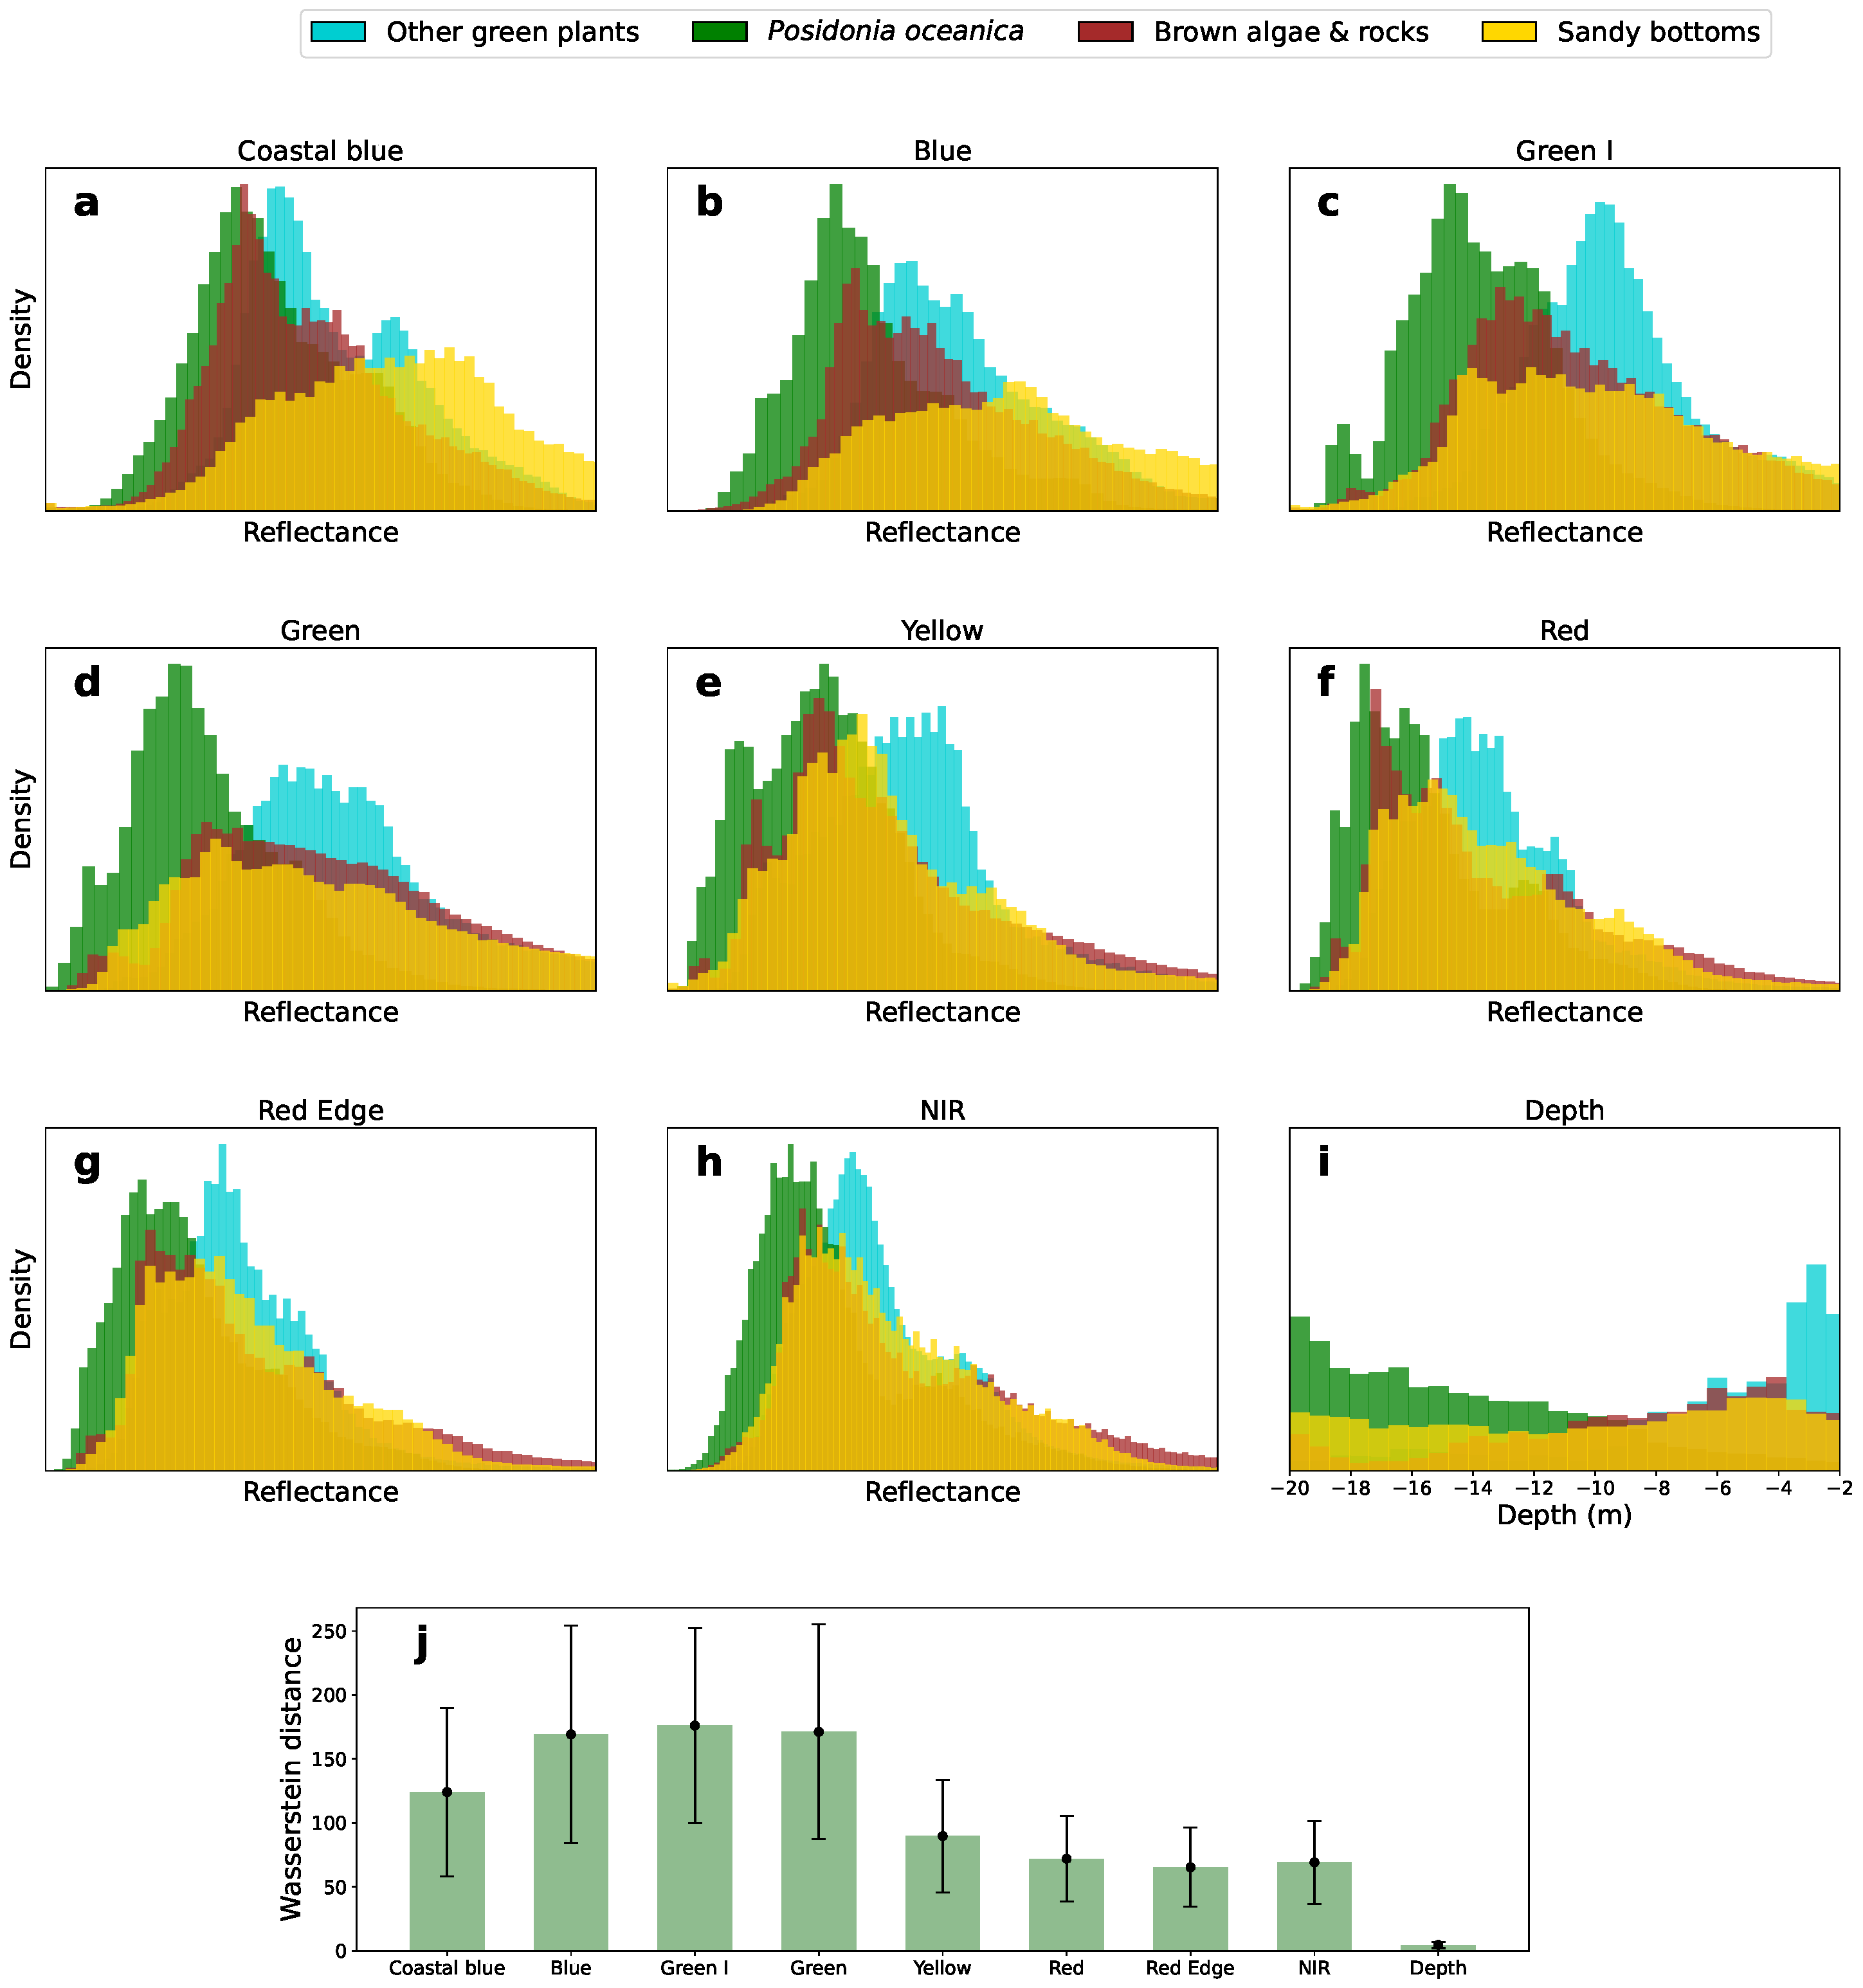
\includegraphics[width=0.95\textwidth]{Figures/Reflectance_histograms_Mallorca_only.pdf}
    \caption{Distribution of response values (surface reflectance) for the
        different processed habitat classes with respect to the different bands
        available from the satellite imagery and depth.}
    \label{fig:reflectance}
\end{figure}

\section{Architecture selection}\label{app:architecture_selection}

We trained the 40 deep learning models as specified in the Methods
section. After training, the performance on both train and validation sets was
compared among the models. Models based on UNET and Linknet clearly
outperformed models based on PSPNet and FPN architectures
(\cref{tab:metrics-architectures}). Despite the similar performance of the
models based on both UNET and Linknet architectures, UNET is a more complex
architecture than Linknet, which translates into a bigger number of trainable
parameters (\cref{tab:parameters-architectures}). Thus, models based on UNET
architecture are more computationally expensive and, in addition, are more
prone to suffer from over-fitting. Thus, we finally selected Linknet as the
main architecture for our models.

\begin{table}[H]
    \centering
    \caption{Performance among all architectures for all backbones based on
        the Intersection over Union metric.}
    \label{tab:metrics-architectures}
    \begin{tabular}{lccccccc}
        \toprule
        \textbf{Architecture} & \textbf{UNET}  & \textbf{Linknet} &
        \textbf{PSPNet}       &
        \textbf{FPN}
        \\
        \midrule
        densenet201           & 91.15          & \textbf{91.51}   & 86.93
                              & 87.97
        \\
        resnet152             & \textbf{92.01} & 91.95            & 86.94
                              & 90.64
        \\
        seresnext101          & 91.52          & \textbf{91.54}   & 85.52
                              & 87.88
        \\
        efficientnetb7        & \textbf{89.27} & 88.65            & 85.99
                              & 87.19
        \\
        inceptionv3           & 89.49          & \textbf{90.59}   & 85.13
                              & 89.33
        \\
        seresnet152           & 91.76          & \textbf{91.83}   & 86.49
                              & 90.48
        \\
        inceptionresnetv2     & 91.85          & \textbf{91.91}   & 86.16
                              & 89.61
        \\
        resnext101            & 92.16          & \textbf{92.5}    & 86.96
                              & 89.09
        \\
        mobilenetv2           & \textbf{89.35} & 89.16            & 83.15
                              & 89.67
        \\
        resnet34              & \textbf{90.44} & 90.14            & 86.12
                              & 90.05
        \\
        \bottomrule
    \end{tabular}
\end{table}

\section{Out-of-sample predicting power and
  robustness}\label{app:out_of_sample}

Because the performance of the different backbones can differ from one
another, with some being better than others in certain situations, we
implemented a pixel-wise consensus algorithm to enhance the robustness and
reliability of model predictions. Basically, the results from all models were
aggregated and the class label with the highest frequency across all
predictions was assigned to the each pixel. Following this algorithm, we tested
different aggregation strategies: selecting all the models (voting\_all),
selecting only the best 3 or 5 models (voting\_top\_3, voting\_top\_5) and
selecting the models that performed better in segmenting each class
individually (voting\_specialists).

\begin{table}[H]
    \centering
    \caption{Number of total parameters among all architectures for all
        backbones (in millions)}
    \label{tab:parameters-architectures}
    \begin{tabular}{lccccccc}
        \toprule
        \textbf{Architecture} & \textbf{UNET} & \textbf{Linknet} \\
        \midrule
        resnet152             & 67.31         & \textbf{63.53}   \\
        mobilenetv2           & 8.04          & \textbf{4.14}    \\
        seresnet152           & 73.95         & \textbf{70.17}   \\
        inceptionv3           & 29.93         & \textbf{26.27}   \\
        densenet201           & 26.39         & \textbf{22.56}   \\
        inceptionresnetv2     & 62.06         & \textbf{57.87}   \\
        seresnext101          & 56.07         & \textbf{52.29}   \\
        efficientnetb7        & 75.05         & \textbf{72.26}   \\
        resnet34              & 24.47         & \textbf{21.65}   \\
        resnext101            & 51.29         & \textbf{47.52}   \\
        \bottomrule
    \end{tabular}
\end{table}

We compared the performance of our Linknet models and consensus strategies
in both the training and out-of-sample test datasets. Regarding the training
set, we observe that some models perform better than others, as expected. At an
individual basis, inceptionresnetv2 and resnext101 are the best-performing
backbones, while efficientnetb7 and densenet201 are the worst-performing ones
(\cref{tab:metrics-train}). The consensus strategies cluster at the first
positions of the ranking, with voting\_top\_3 and voting\_top\_5 occupying the
two first positions. Interestingly, we observe that efficientnetb7 is the
best-performing backbone in the test set, followed by voting\_all and
inceptionresnetv2 (\cref{tab:metrics-test}). This suggests that efficientnetb7
is one of the most robust models, with higher generalization power. At any
rate, we observe that it is closely followed by the voting\_all consensus
strategy. Here we must emphasize that while the mask class is considered during
training, it is omitted during evaluation and prediction phases to focus solely
on the specified classes of interest. Consequently, this contributes to the
observed differences in IoU values between \cref{tab:metrics-architectures} and
\cref{tab:metrics-train,tab:metrics-test}.

\begin{table}[H]
    \centering
    \caption{Performance metrics for all models based on Linknet
        architecture in the training dataset}
    \label{tab:metrics-train}
    \begin{tabular}{lccccccc}
        \toprule
        Backbone                & IoU            & f1             & Kappa
                                & Precision      & Recall         &
        Accuracy
        \\
        \midrule
        \textbf{voting\_top\_3} & \textbf{89.57} & \textbf{94.01} &
        \textbf{80.72}          & \textbf{94.79} & \textbf{94.37} &
        \textbf{94.28}                                                    \\
        voting\_top\_5          & 89.01          & 93.64          & 80.12
                                & 94.59          & 94.01          & 93.9
        \\
        inceptionresnetv2       & 88.95          & 93.72          & 81.35
                                & 94.3           & 93.99          & 93.9
        \\
        resnext101              & 88.46          & 93.27          & 78.48
                                & 94.22          & 93.65          & 93.55
        \\
        resnet152               & 88.34          & 93.23          & 78.72
                                & 94.12          & 93.62          & 93.54
        \\
        voting\_all             & 88.22          & 93.13          & 78.63
                                & 94.24          & 93.56          & 93.44
        \\
        voting\_specialists     & 88.22          & 93.21          & 79.27
                                & 94.2           & 93.57          &
        93.46
        \\
        mobilenetv2             & 88.01          & 93.16          & 80.74
                                & 93.78          & 93.37          & 93.28
        \\
        resnet34                & 86.43          & 91.95          & 75.29
                                & 93.12          & 92.47          & 92.33
        \\
        inceptionv3             & 85.96          & 91.74          & 77.56
                                & 92.88          & 92.09          & 92.04
        \\
        seresnet152             & 85.74          & 91.54          & 76.36
                                & 92.94          & 91.91          & 91.79
        \\
        seresnext101            & 85.65          & 91.55          & 76.2
                                & 92.75          & 91.92          & 91.77
        \\
        efficientnetb7          & 84.56          & 90.79          & 72.95
                                & 91.86          & 91.35          & 91.19
        \\
        densenet201             & 82.21          & 89.04          & 69.72
                                & 90.99          & 89.67          & 89.48
        \\
        \hdashline
        Median                  & 88.12          & 93.16          & 78.56
                                & 93.95          & 93.47          & 93.36
        \\
        \bottomrule
    \end{tabular}
\end{table}

Overall, we note that the relative performance of the model in the
out-of-sample test set is significantly reduced in comparison with the training
set, although the absolute performance is still considerable. This, indeed, is
expected, as the habitat classes of the out-of-sample test are not formed by
exactly the same sub-categories that in the training set. Furthermore, there is
a huge environmental variability and intrinsic noise in the overall framework
proposed here: the relative position of the satellite with respect to the sun
and the earth at the time of each image acquisition, the specific atmospheric
and marine conditions, the fact that some species forming the habitat classes
are seasonal, etc.

\begin{table}[H]
    \centering
    \caption{Performance metrics for all models based on Linknet
        architecture in the out-of-sample test dataset}
    \label{tab:metrics-test}
    \begin{tabular}{lcccccc}
        \toprule
        Backbone                & IoU            & f1             & Kappa
                                & Precision      & Recall         &
        Accuracy
        \\
        \midrule
        \textbf{efficientnetb7} & \textbf{62.19} & \textbf{73.05} &
        \textbf{54.34}          & 76.1           & 74.78          & 74.62
        \\
        \textbf{voting\_all}    & 61.97          & 72.77          & 53.7
                                & \textbf{76.74} & \textbf{75.02} &
        \textbf{74.88}                                                    \\
        inceptionresnetv2       & 61.80          & 72.69          & 52.8
                                & 75.31          & 74.87          & 74.7
        \\
        voting\_top\_5          & 61.35          & 72.38          & 53.11
                                & 76.29          & 74.38          & 74.25
        \\
        voting\_specialists     & 61.10          & 71.92          & 52.2
                                & 75.93          & 74.47          &
        74.37
        \\
        voting\_top\_3          & 60.88          & 71.92          & 52.03
                                & 75.94          & 74.08          & 73.94
        \\
        mobilenetv2             & 60.87          & 72.01          & 51.74
                                & 74.40          & 74.12          & 73.97
        \\
        seresnext101            & 60.58          & 71.82          & 52.02
                                & 75.01          & 73.57          & 73.35
        \\
        resnext101              & 60.46          & 71.68          & 51.64
                                & 75.39          & 73.68          & 73.50
        \\
        seresnet152             & 60.14          & 71.48          & 52.77
                                & 75.58          & 72.94          & 72.67
        \\
        inceptionv3             & 59.65          & 70.82          & 50.66
                                & 73.81          & 72.85          & 72.65
        \\
        densenet201             & 59.2           & 70.69          & 51.57
                                & 75.37          & 72.01          & 71.83
        \\
        resnet152               & 57.58          & 69.16          & 48.89
                                & 73.04          & 71.00          &
        70.91
        \\
        resnet34                & 57.54          & 69.2           & 47.38
                                & 72.54          & 71.32          & 71.16
        \\
        \hdashline
        Median                  & 60.73          & 71.87          & 52.03
                                & 75.38          & 73.88          & 73.72
        \\
        \bottomrule
    \end{tabular}
\end{table}

\subsection{Understanding model performance}

\begin{table}[H]
    \centering
    \caption{Performance in segmenting each habitat class individually,
        measured by Intersection over Union, for all models in training and
        out-of-sample test datasets.}
    \label{tab:metrics_classes}
    \begin{tabular}{lcccc|cccc}
        \toprule
                            & \multicolumn{4}{c}{Training dataset} &
        \multicolumn{4}{|c}{Test
            dataset}

        \\
        \midrule
        Method              & PO                                   & OGP
                            & SB                                   & BAR
                            & PO                                   & OGP
                            & SB
                            & BAR

        \\
        \midrule
        densenet201         & 88.69                                & 69.9
                            & 75.35                                & 66.25
                            & 72.48                                & 5.44
                            &
        55.12               & 38.24

        \\
        efficientnetb7      & 90.26                                & 69.56
                            & 77.37                                & 74.66
                            & 76.99                                & 3.86
                            &
        \textbf{56.31}      & 40.59

        \\
        inceptionresnetv2   & \textbf{92.61}                       &
        \textbf{85.81}      & 83.63                                & 81.17
                            &
        \textbf{77.34}      & 3.72                                 & 53.85
                            & \textbf{41.17}
        \\
        inceptionv3         & 90.8                                 & 73.6
                            & 80.82                                & 75.57
                            & 75.79                                & 3.79
                            &
        50.99               & 38.21

        \\
        mobilenetv2         & 92.05                                & 83.6
                            & 81.49                                & 81.44
                            & 76.76                                &
        \textbf{5.49}       & 53.16                                & 37.27

        \\
        resnet152           & 91.87                                & 85.61
                            & 82.79                                &
        \textbf{81.7}       & 71.54                                &
        2.92                & 51.04                                & 37.92

        \\
        resnet34            & 90.8                                 & 82.7
                            & 80.78                                & 75.84
                            & 73.11                                & 3.37
                            &
        49.71               & 35.7

        \\
        resnext101          & 92.09                                & 85.78
                            & \textbf{83.65}                       & 79.56
                            & 75.74                                &
        4.39                & 52.92                                & 39.6

        \\
        seresnet152         & 90.87                                & 75.98
                            & 79.63                                & 74.45
                            & 73.09                                & 4.82
                            &
        55.65               & 40.4

        \\
        seresnext101        & 90.67                                & 77.45
                            & 78.53                                & 76.53
                            & 75.61                                & 4.09
                            &
        53.69               & 39.49

        \\
        \midrule
        voting\_all         & 91.97                                & 85.29
                            & 82.2                                 & 81.54
                            & 77.30                                &
        \textbf{4.24}
                            & \textbf{54.50}                       &
        \textbf{41.99}
        \\
        voting\_top\_3      & \textbf{92.79}                       &
        \textbf{87.28}      & \textbf{84.72}                       &
        \textbf{83.01}      & 76.25                                & 4.12
                            & 53.11                                & 40.57
        \\
        voting\_top\_5      & 92.5                                 & 86.1
                            & 83.54                                & 82.53
                            & 76.18                                & 4.13
                            &
        54.44               & 41.71

        \\
        voting\_specialists & 92.01                                & 86.78
                            & 82.38                                & 80.21
                            & \textbf{77.31}                       &
        4.22                & 51.88                                & 40.69

        \\
        \bottomrule
        Area in (km$^2$)    & 359.96                               & 29.31
                            & 139.46                               & 63.82
                            & 156.12                               & 18.17
                            &
        80.59               & 36.96

        \\
    \end{tabular}
\end{table}

We then studied the performance of the model on segmenting each of the
ecological habitats individually. We observed the emergence of ``specialists'':
in the training set, inceptionresnet outperforms in segmenting
\textit{Posidonia oceanica} meadows and Other green plants, resnext101 is
better suited for mapping Sandy bottoms while resnet152 shows enhanced
performance for detecting Brown algae \& rocks (\cref{tab:metrics_classes}).

However, the results change when looking at the test dataset. This somehow
explains why the voting\_all consensus method outperforms the voting\_smart
one. We also note that the performance of the model with respect to Other green
plants is drastically reduced in the test set, which undoubtedly affect the
overall performance of the model shown in \cref{tab:metrics-test}.

To further understand this drastic loss of performance on segmenting the
``Other green plants'' class, we computed the confusion matrix for the model
(voting\_all from now on) predictions (\cref{fig:confusion_matrix}). In the
training dataset there is already a significant difference between the
performance in segmenting \textit{Posidonia oceanica} meadows, with 99.5\% True
Positives (TP) and the other classes, with 89.4\% TP for Other green plants,
84.5\% TP for Brown algae \& rocks and 83.6\% TP for Sandy Bottoms
(\cref{fig:confusion_matrix} a). At any rate, those differences clearly
increase in the out-of-sample test set. While the segmentation of
\textit{Posidonia oceanica} meadows keeps a remarkable 94.6\% TP, with a still
low FP rate, the TP rate for the other classes is reduced
(\cref{fig:confusion_matrix} b). Specifically, a significant part of the pixels
that were categorized by the ground truth data as Other green plants, Brown
algae \& rocks or Sandy bottoms are being classified by the model as
\textit{Posidonia oceanica} meadows. This is the reason for the very low IoU
score of the Other green plant class in the testing set and the overall IoU
decrease in all classes. In addition, we can also observe that the area of each
class is significantly reduced in the test set in comparison with the training
set (\cref{fig:confusion_matrix}c-d, sum over rows).

\begin{figure}[H]
    \centering
    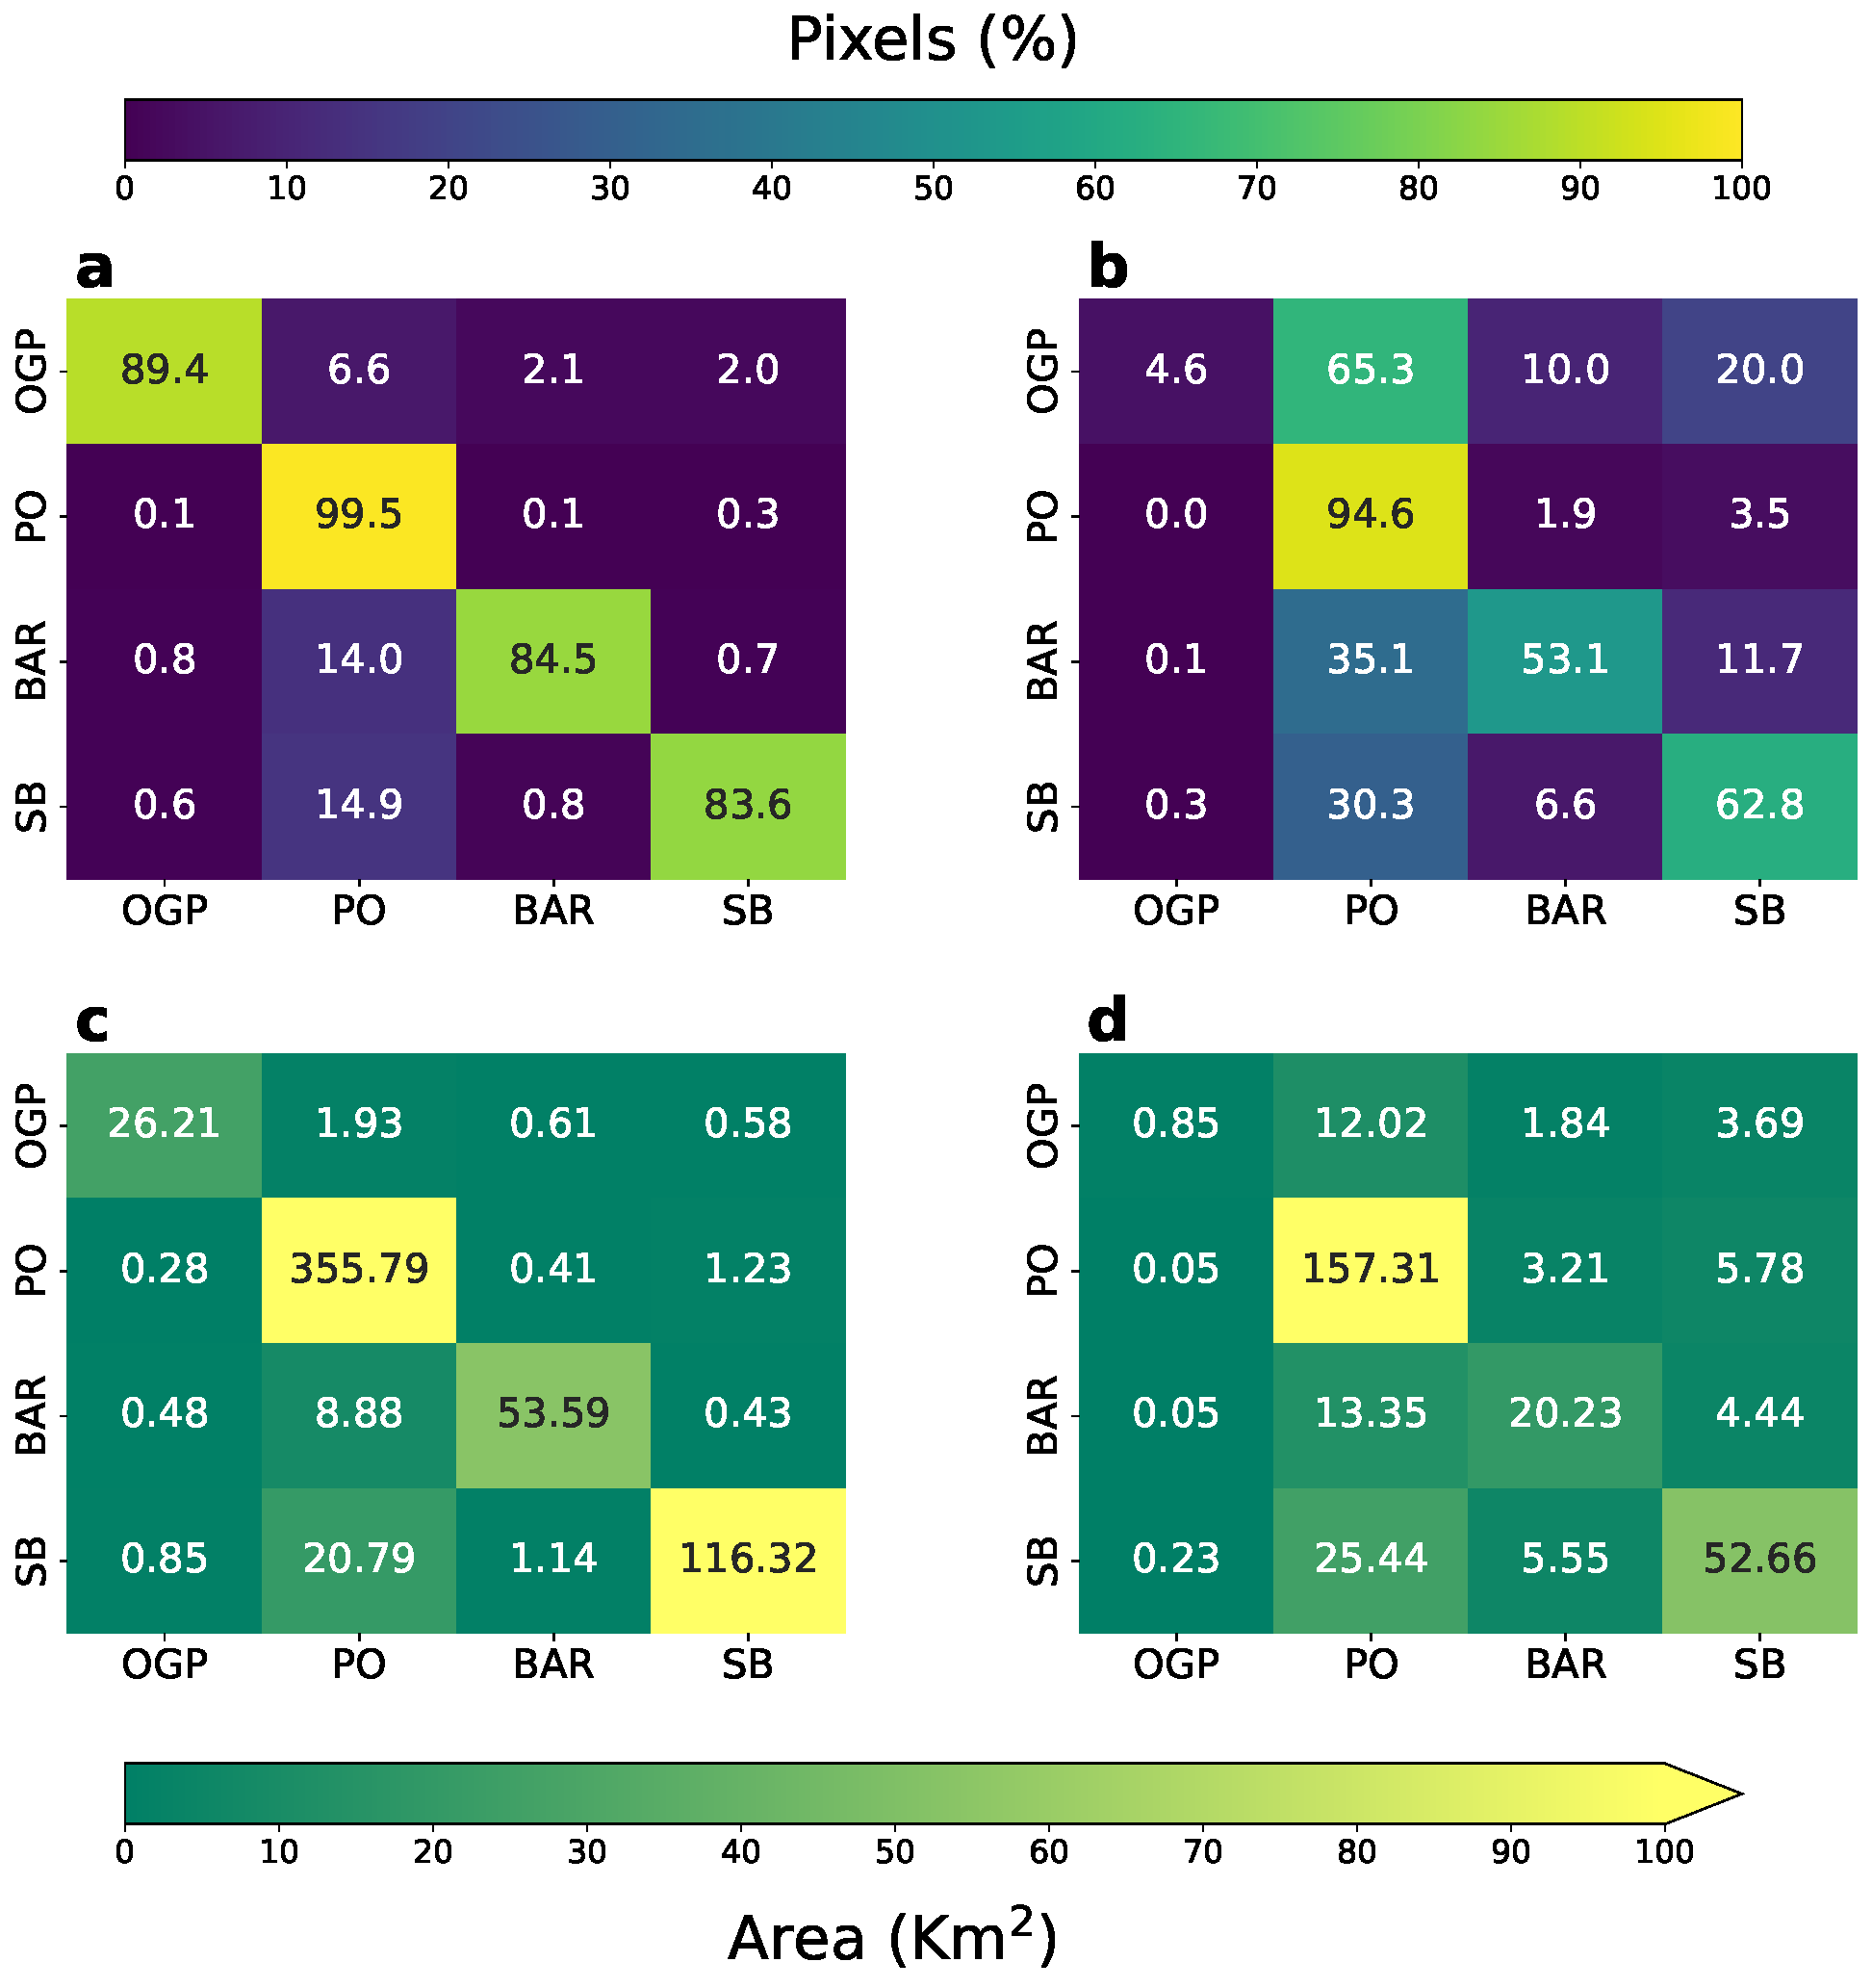
\includegraphics[width=\textwidth]{Figures/Confusion_matrix.pdf}
    \caption{Confusion matrix for train (a) and out-of-sample test (b)
        dataset. Confusion matrix for the predicted area in train (c) and
        out-of-sample
        test (d) datasets.}
    \label{fig:confusion_matrix}
\end{figure}

To better understand this behavior, we compared the response values of each
class between train and test datasets. In principle, the distribution of
response values for a given class in the test set should be similar to the
distribution of that class in the training set. This is indeed the rationale
behind the use of correlative models. Of course, this distributions should be
similar in a high dimensional space that we are not able to visualize. At any
rate, to gain some understanding, we computed the wasserstein distance between
the distribution of response values in train and test for the Blue, Green and
Green I bands, i.e. the most influential bands, as previously found.

The results revealed that the distribution of response values for the Other
green plants class in the test dataset is much more similar to the
\textit{Posidonia oceanica} distribution of response values in the train set
than to its own class (\cref{fig:similarity_train_test_classes}), specially for
Green I and Green bands (\cref{fig:similarity_train_test_classes} b-c). Then it
is not surprising that the model classifies all those samples as
\textit{Posidonia oceanica}. Indeed, because of the great seasonality and
natural variability of some of the species conforming the Other green plants
class, the real habitat class present at the time of the satellite image
acquisition could deviate from the initial one present at sonar-based
classification. Similarly, there are some mixed sub-classes
such as ``Photophilic algae on stone with \textit{Posidonia oceanica}" which
further increase the probability of the previous argument taking place. That
would explain the fact that the distribution of the response values for the
``Other green plants'' class in the test dataset is more similar to the
\textit{Posidonia oceanica} distribution in the training set than to its own
class in the training set. So, in summary, it is plausible that some of the
model predictions that are supposed to be incorrect, were indeed correct.

\begin{figure}[H]
    \centering

    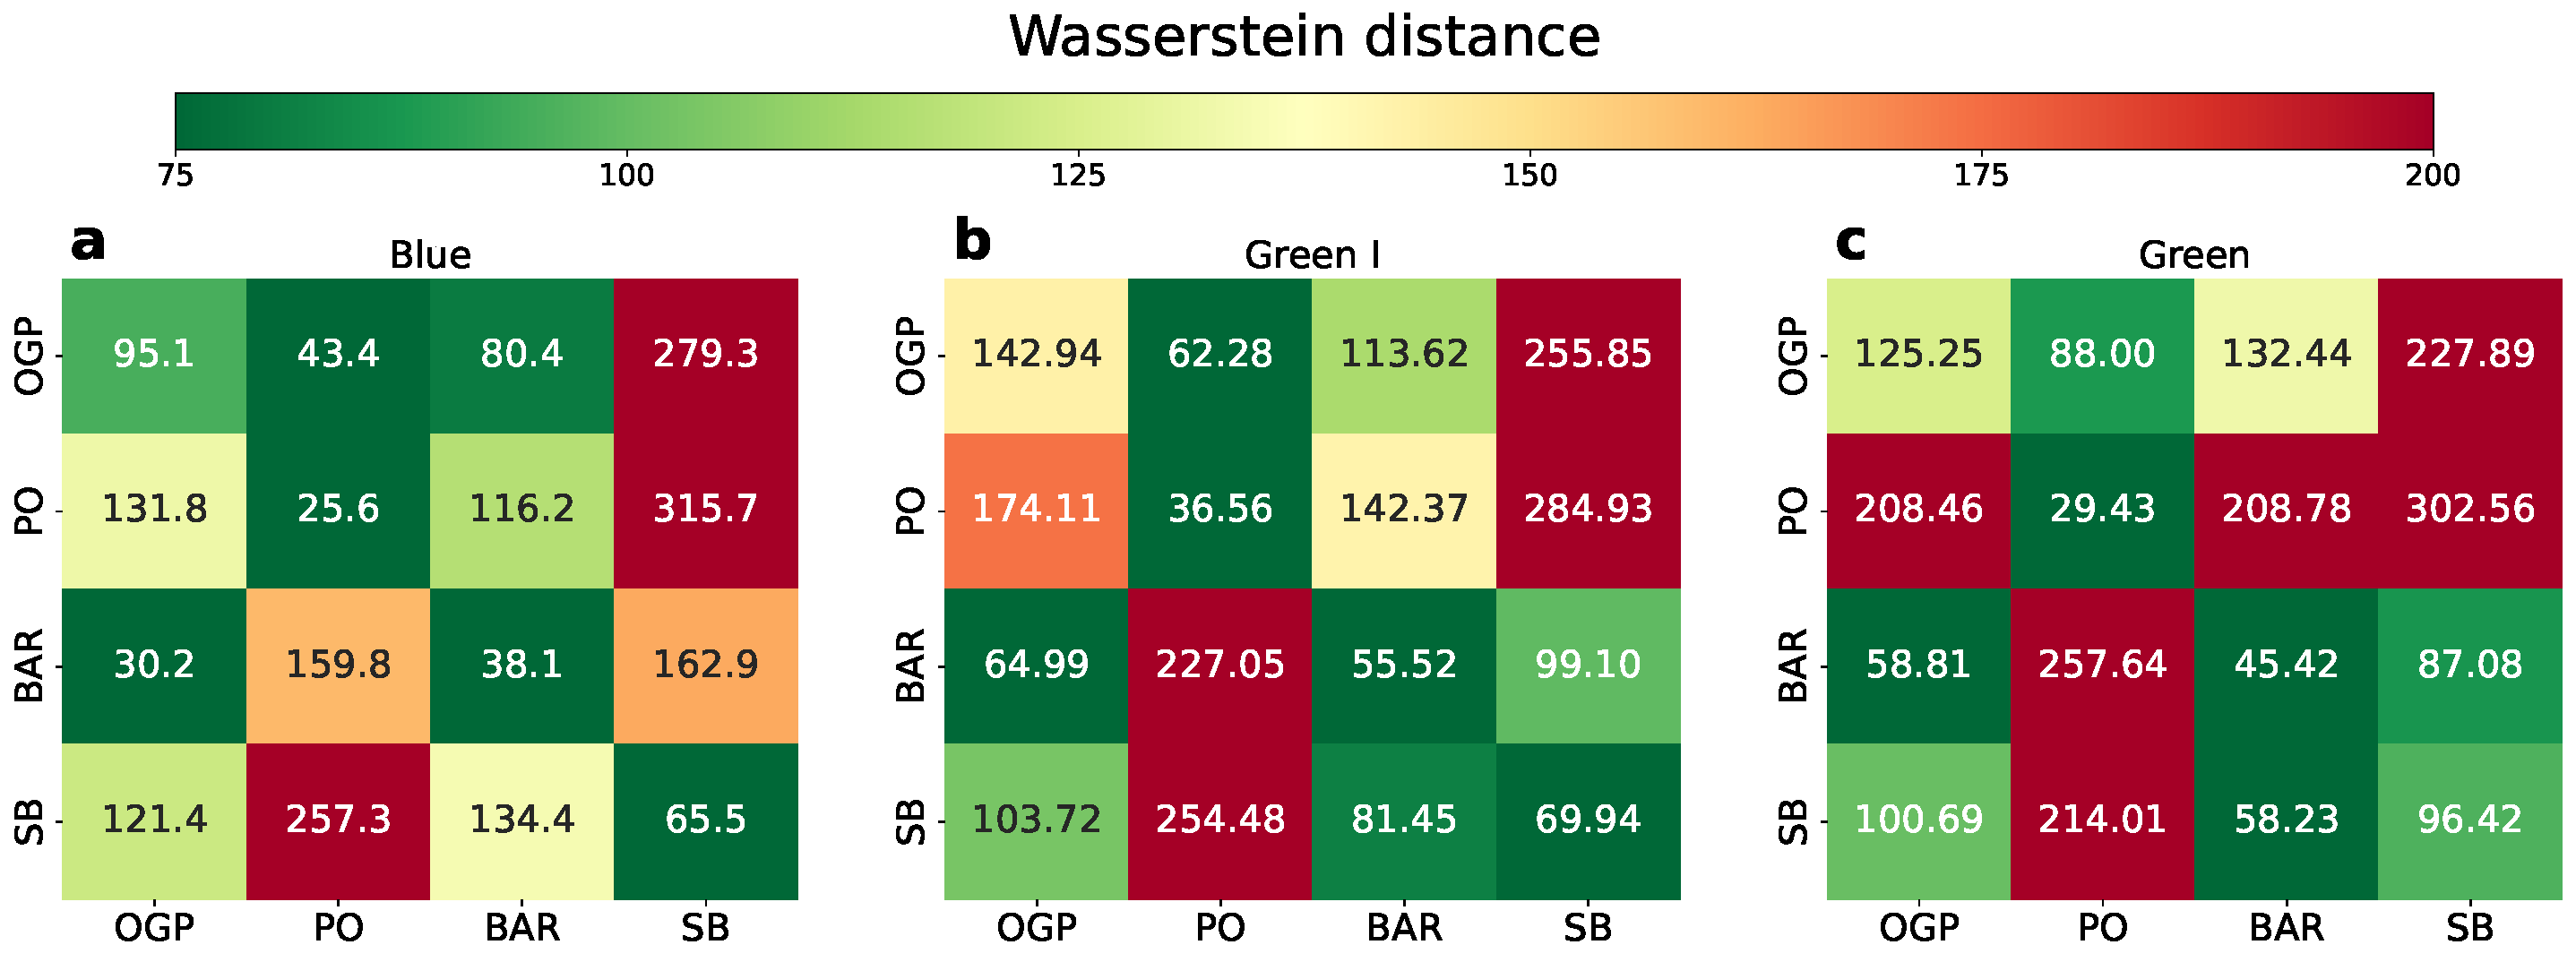
\includegraphics[width=\textwidth]{Figures/Wasserstein_distance_by_Classes_&_Datasets.pdf}
    \caption{Wasserstein distance between Train and Test datasets for Blue
        (a), Green I (b) and Green (c) bands.}
    \label{fig:similarity_train_test_classes}
\end{figure}

All the analysis on model performance done up to this point were based on
\textbf{mean} results over the training and out-of-sample test datasets, which
are based on 21 images each. Now we analyze the performance of the model
predictions in each image individually (\cref{tab:metrics_img}). We observe
that there is a great variability in model performance within each dataset. In
the training set, $60\%$ of the images are segmented with IoU$>90\%$ and $30\%$
with IoU$>80\%$. The resting 2 images, however, are segmented with ``only''
around $64\%$ IoU score, overlapping with the out-of-sample test dataset
(\cref{tab:metrics_img}). In the test set, $15\%$ of the images are segmented
with IoU$>80\%$, $20\%$ with IoU$>70\%$ and $45\%$ with IoU$>50\%$. The resting
4 images are segmented with an IoU score of around $40\%$. In any case, the
accuracy of all segmentations are always over $50\%$, much above the threshold
for random segmentation of $25\%$ (recall it is a 4-class classification
problem).

These results present two interesting insights. First, the model is able to
segment some images in the test set with very high performance ($15\%$ of the
images). Recall this is not a usual testing set, but we have only trained the
model in a given island (Mallorca) and tested it in 3 other islands (Menorca,
Ibiza and Formentera), not controlling for neither weather or
satellite-position variability. Second, we observe that 2 images in the
training test are segmented with rather ``low'' performance, situating at the
middle of the testing set in the performance ranking
(\cref{tab:metrics_img}). Interestingly, those are images situated in the
``Serra de Tramuntana'', the mountain range in Mallorca. The sea bottom in this
area is characterized by a rocky substrate where depth increases rapidly.
Indeed, we can observe that the images that are segmented with higher
performance in the test set (Formentera\_24\_july\_2022 to
Sur\_Ibiza\_20\_july\_2022) are precisely characterized by more sandy and clear
sea bottoms with slowly increasing depths, while the rest are rather rocky with
rapidly increasing depth (\cref{tab:metrics_img}). This insights can help in
taking future steps to develop a general model for segmenting sea habitats in
the whole Mediterranean sea.

\begin{table}[H]
    \centering
    \caption{Performance metrics for voting\_all model in segmenting
        individual images from training and testing datasets.}
    \label{tab:metrics_img}
    \resizebox{\columnwidth}{!}{%
        \begin{tabular}{lllllllll}
            \toprule
            \textbf{Image Name}                    & \textbf{IoU}        &
            \textbf{f1}                            & \textbf{Kappa}      &
            \textbf{Precision}                     & \textbf{Recall}     &
            \textbf{Accuracy}                      & \textbf{Area (Km²)}
                                                   & \textbf{Dataset}
            \\ \midrule
            PortoColom\_CalaMillor\_22\_july\_2022 & 94.77               &
            97.27
                                                   & 94.21               &
            97.31
                                                   & 97.3                &
            97.24
                                                   & 28.22               &
            {\color[HTML]{66c2a5} Train}
            \\
            Es\_trenc\_25\_july\_2022              & 93.56               &
            96.53
                                                   & 87.1                &
            96.81
                                                   & 96.57               &
            96.54
                                                   & 12.65               &
            {\color[HTML]{66c2a5} Train}
            \\
            Capdepera\_22\_july\_2022              & 93.23               &
            96.43
                                                   & 94.04               &
            96.52
                                                   & 96.47               &
            96.37
                                                   & 15.89               &
            {\color[HTML]{66c2a5} Train}
            \\
            Pollença\_6\_july\_2021                & 92.78               &
            96.06
                                                   & 86.42               & 96.3
                                                   & 96.27               &
            96.22
                                                   & 26.02               &
            {\color[HTML]{66c2a5} Train}
            \\
            CalaPi\_CalaFiguera\_23\_july\_2022    & 92.34               &
            95.83
                                                   & 90.89               &
            96.12
                                                   & 96.02               &
            95.96
                                                   & 36.58               &
            {\color[HTML]{66c2a5} Train}
            \\
            Alcudia\_25\_july\_2022                & 91.97               &
            95.52
                                                   & 79.92               &
            95.92
                                                   & 95.83               &
            95.81
                                                   & 76.18               &
            {\color[HTML]{66c2a5} Train}
            \\
            Capdepera\_20\_july\_2021              & 91.37               &
            95.36
                                                   & 92.31               & 95.6
                                                   & 95.43               &
            95.34
                                                   & 15.89               &
            {\color[HTML]{66c2a5} Train}
            \\
            Pollença\_23\_may\_2020                & 91.12               &
            94.99
                                                   & 81.0                &
            95.44
                                                   & 95.39               &
            95.33
                                                   & 24.7                &
            {\color[HTML]{66c2a5} Train}
            \\
            CalaPi\_CalaFiguera\_29\_july\_2021    & 90.87               &
            94.95
                                                   & 90.16               &
            95.47
                                                   & 95.15               &
            95.09
                                                   & 36.53               &
            {\color[HTML]{66c2a5} Train}
            \\
            Banyalbufar\_Soller\_23\_july\_2021    & 90.38               &
            94.89
                                                   & 90.71               &
            95.07
                                                   & 94.94               &
            94.81
                                                   & 8.88                &
            {\color[HTML]{66c2a5} Train}
            \\
            Dragonera\_Toro\_23\_july\_2021        & 90.06               &
            94.63
                                                   & 90.71               &
            94.82
                                                   & 94.76               & 94.5
                                                   & 11.93               &
            {\color[HTML]{66c2a5} Train}
            \\
            Dragonera\_Toro\_22\_july\_2022        & 90.05               &
            94.65
                                                   & 90.62               &
            94.84
                                                   & 94.77               &
            94.49
                                                   & 11.87               &
            {\color[HTML]{66c2a5} Train}
            \\
            Pollença\_21\_july\_2022               & 89.82               &
            94.01
                                                   & 77.29               &
            94.83
                                                   & 94.7                &
            94.65
                                                   & 26.05               &
            {\color[HTML]{66c2a5} Train}
            \\
            PortoColom\_CalaMillor\_27\_july\_2021 & 88.91               &
            93.99
                                                   & 86.49               &
            94.44
                                                   & 94.14               &
            94.08
                                                   & 28.22               &
            {\color[HTML]{66c2a5} Train}
            \\
            Alcudia\_22\_july\_2021                & 86.06               &
            91.52
                                                   & 63.17               &
            93.14
                                                   & 92.51               &
            92.47
                                                   & 75.69               &
            {\color[HTML]{66c2a5} Train}
            \\
            Alcudia\_21\_may\_2020                 & 84.62               &
            90.44
                                                   & 58.93               &
            92.69
                                                   & 91.34               & 91.3
                                                   & 73.63               &
            {\color[HTML]{66c2a5} Train}
            \\
            Dragonera\_Banyalbufar\_10\_july\_2021 & 83.97               &
            91.04
                                                   & 85.27               &
            92.17
                                                   & 91.11               &
            90.87
                                                   & 7.09                &
            {\color[HTML]{66c2a5} Train}
            \\
            Formentera\_24\_july\_2022             & 82.57               &
            89.53
                                                   & 82.24               &
            89.73
                                                   & 89.74               &
            88.55
                                                   & 28.96               &
            {\color[HTML]{fc8d62} Test}
            \\
            Formentera\_18\_july\_2021             & 82.54               &
            89.52
                                                   & 82.27               & 89.9
                                                   & 89.84               &
            88.68
                                                   & 28.99               &
            {\color[HTML]{fc8d62} Test}
            \\
            Palma\_7\_july\_2022                   & 82.42               &
            90.03
                                                   & 81.53               &
            91.59
                                                   & 90.1                &
            88.99
                                                   & 57.4                &
            {\color[HTML]{66c2a5} Train}
            \\
            Sur\_Oeste\_Menorca\_09\_July\_2021    & 82.12               &
            88.25
                                                   & 58.03               &
            87.84
                                                   & 89.5                &
            89.55
                                                   & 10.87               &
            {\color[HTML]{fc8d62} Test}
            \\
            North\_Cabrera\_19\_july\_2022         & 77.78               &
            86.24
                                                   & 49.14               &
            87.42
                                                   & 85.54               &
            85.54
                                                   & 1.37                &
            {\color[HTML]{fc8d62} Test}
            \\
            Sur\_Oeste\_Menorca\_29\_July\_2022    & 75.14               &
            84.15
                                                   & 36.85               &
            88.46
                                                   & 81.84               &
            80.29
                                                   & 16.4                &
            {\color[HTML]{fc8d62} Test}
            \\
            Sur\_Ibiza\_18\_july\_2021             & 70.41               &
            79.92
                                                   & 51.71               &
            80.02
                                                   & 81.73               &
            82.14
                                                   & 21.47               &
            {\color[HTML]{fc8d62} Test}
            \\
            Sur\_Ibiza\_20\_july\_2022             & 70.11               &
            79.64
                                                   & 50.29               &
            79.84
                                                   & 81.55               &
            81.97
                                                   & 22.52               &
            {\color[HTML]{fc8d62} Test}
            \\
            South\_Cabrera\_23\_july\_2022         & 64.89               & 77.3
                                                   & 47.39               &
            81.76
                                                   & 76.02               & 76.0
                                                   & 1.45                &
            {\color[HTML]{fc8d62} Test}
            \\
            Banyalbufar\_Soller\_17\_july\_2022    & 64.49               &
            76.47
                                                   & 54.73               &
            84.17
                                                   & 79.5                & 79.4
                                                   & 8.83                &
            {\color[HTML]{66c2a5} Train}
            \\
            Dragonera\_Banyalbufar\_29\_july\_2022 & 63.14               & 76.1
                                                   & 62.49               &
            85.53
                                                   & 76.27               &
            75.88
                                                   & 7.25                &
            {\color[HTML]{66c2a5} Train}
            \\
            Este\_Ibiza\_18\_july\_2021            & 62.28               & 73.4
                                                   & 43.37               &
            77.75
                                                   & 76.52               &
            76.53
                                                   & 13.19               &
            {\color[HTML]{fc8d62} Test}
            \\
            Este\_Ibiza\_24\_july\_2022            & 61.53               &
            72.59
                                                   & 42.15               & 77.8
                                                   & 75.62               &
            75.67
                                                   & 13.21               &
            {\color[HTML]{fc8d62} Test}
            \\
            Oeste\_Ibiza\_14\_july\_2022           & 59.56               &
            73.26
                                                   & 54.19               &
            76.74
                                                   & 75.17               &
            75.92
                                                   & 7.72                &
            {\color[HTML]{fc8d62} Test}
            \\
            Oeste\_Ibiza\_18\_july\_2021           & 58.9                &
            72.63
                                                   & 53.26               &
            76.26
                                                   & 74.69               &
            75.59
                                                   & 7.75                &
            {\color[HTML]{fc8d62} Test}
            \\
            Sur\_Este\_Menorca\_29\_July\_2022     & 58.0                &
            69.34
                                                   & 57.21               &
            67.93
                                                   & 74.34               &
            75.16
                                                   & 16.15               &
            {\color[HTML]{fc8d62} Test}
            \\
            Sur\_Este\_Menorca\_02\_July\_2021     & 57.01               &
            68.53
                                                   & 55.82               &
            71.64
                                                   & 73.55               &
            74.38
                                                   & 16.42               &
            {\color[HTML]{fc8d62} Test}
            \\
            Norte\_Ibiza\_18\_july\_2022           & 53.01               &
            68.57
                                                   & 53.45               &
            70.57
                                                   & 69.52               &
            69.21
                                                   & 4.27                &
            {\color[HTML]{fc8d62} Test}
            \\
            Norte\_Ibiza\_18\_july\_2021           & 50.03               &
            66.05
                                                   & 49.13               &
            71.43
                                                   & 66.85               &
            67.13
                                                   & 4.4                 &
            {\color[HTML]{fc8d62} Test}
            \\
            Norte\_Menorca\_20\_July\_2022         & 43.32               & 55.8
                                                   & 43.98               & 69.5
                                                   & 58.77               &
            58.33
                                                   & 13.85               &
            {\color[HTML]{fc8d62} Test}
            \\
            Este\_Menorca\_19\_July\_2021          & 42.26               &
            56.51
                                                   & 42.5                &
            61.63
                                                   & 60.13               &
            60.21
                                                   & 25.49               &
            {\color[HTML]{fc8d62} Test}
            \\
            Este\_Menorca\_15\_July\_2022          & 38.35               &
            52.87
                                                   & 36.78               &
            63.33
                                                   & 57.53               &
            57.42
                                                   & 25.95               &
            {\color[HTML]{fc8d62} Test}
            \\
            Norte\_Menorca\_29\_July\_2021         & 38.28               & 51.3
                                                   & 37.52               &
            67.92
                                                   & 54.69               &
            54.37
                                                   & 14.23               &
            {\color[HTML]{fc8d62} Test}
            \\ \bottomrule
        \end{tabular}%
    }
\end{table}

\section{Effect of depth on model performance}\label{app:depth}

Finally, we studied the effect of depth in model performance, focusing on
the test set. We observe that, in general, model performance is rather
independent on depth (\cref{fig:IoU_class_depth} a). Interestingly, we observe
that the \textit{Posidonia oceanica} class consistently exhibits the highest
IoU values across all depths compared to other classes. This noteworthy trend
may be attributed to the abundance of \textit{Posidonia oceanica} samples
(\cref{fig:IoU_class_depth} b), suggesting that the model's performance excels
in accurately identifying and delineating Posidonia in underwater environments.

\begin{figure}[H]
    \centering
    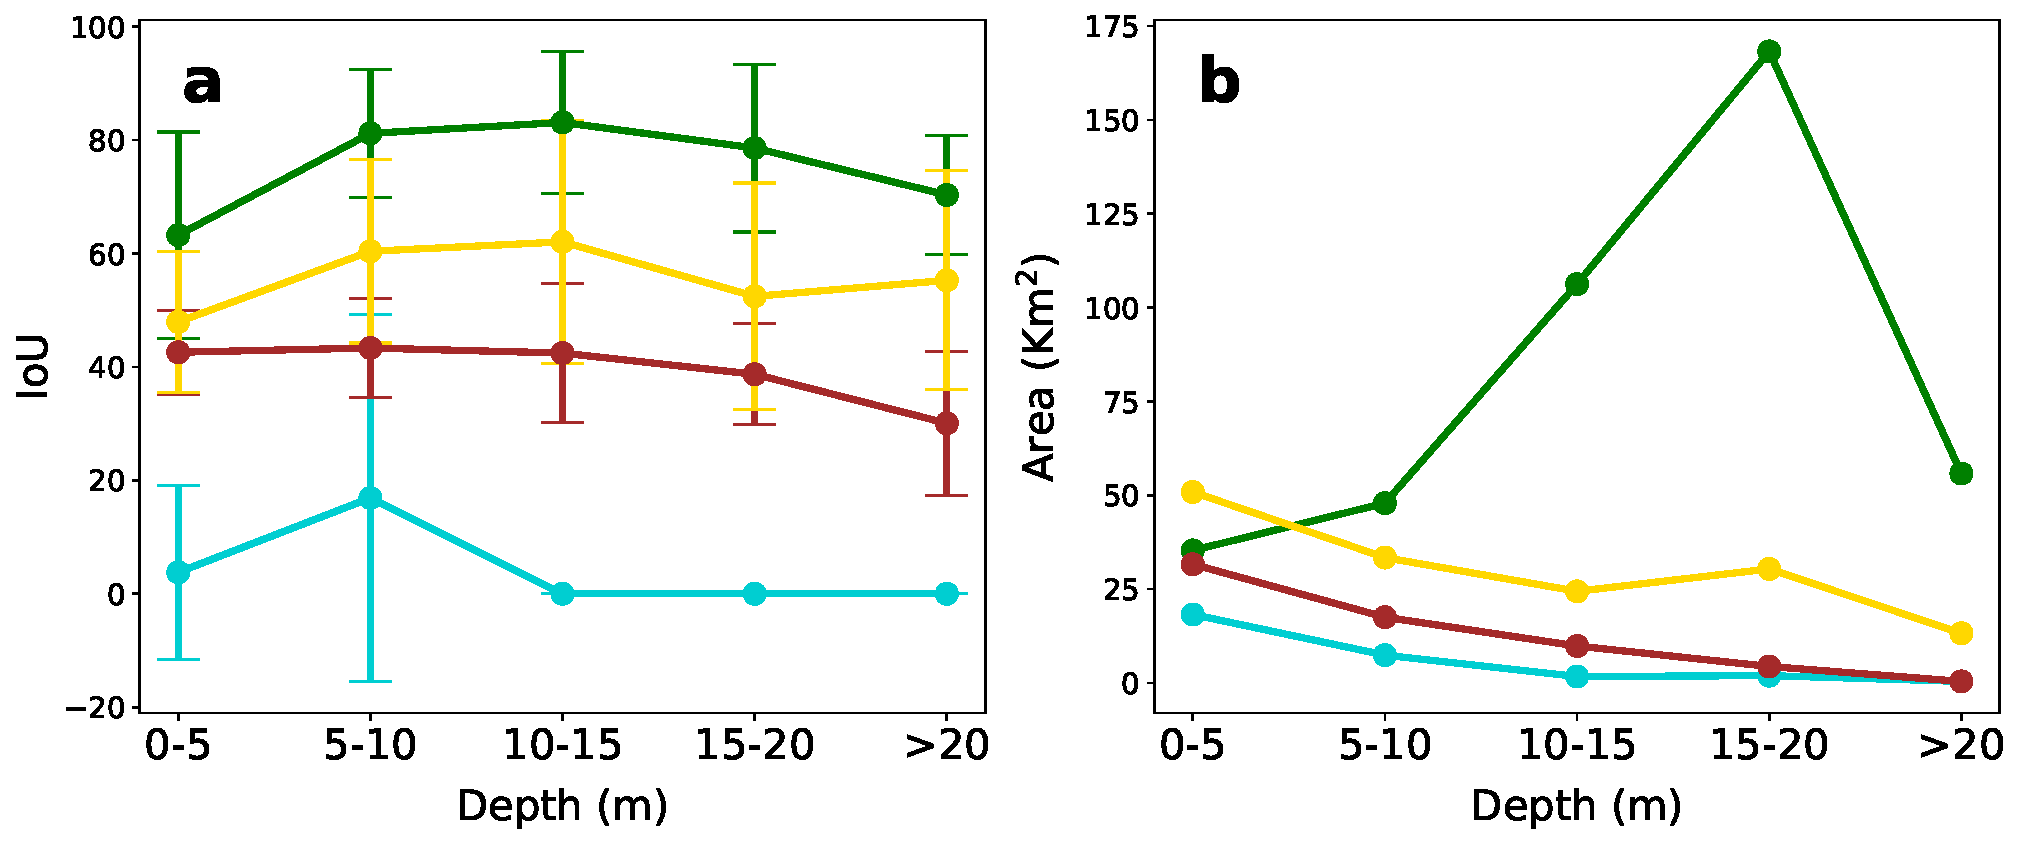
\includegraphics[width=\textwidth]{Figures/IoU_class_depth.pdf}
    \caption{(a) Performance of voting\_all model as function of the depth
        of classified pixels. (b) Area of samples contained in each depth range
        for the
        different habitat classes.}
    \label{fig:IoU_class_depth}
\end{figure}

\begin{table}[H]
    \centering
    \caption{Performance metrics for voting\_all model in segmenting
        individual images from previous training and testing datasets.}
    \label{tab:metrics_img_final}
    \resizebox{\columnwidth}{!}{%
        \begin{tabular}{lcccccccc}
            \toprule
            \textbf{Image Name}                    & \textbf{IoU}
                                                   &
            \textbf{f1}                            & \textbf{Kappa}
                                                   &
            \textbf{Precision}                     & \textbf{Recall}
                                                   &
            \textbf{Accuracy}                      & \textbf{Area (Km²)}
                                                   & \textbf{Dataset}

            \\ \midrule
            Formentera\_18\_july\_2021             & 98.50
                                                   & 99.24
                                                   & 98.50
                                                   & 99.25
                                                   & 99.25
                                                   & 99.25
                                                   & 29.07
                                                   & {\color[HTML]{fc8d62}
                    Test}
            \\
            Formentera\_24\_july\_2022             & 98.42
                                                   & 99.20
                                                   & 98.43
                                                   & 99.20
                                                   & 99.20
                                                   & 99.20
                                                   & 29.04
                                                   & {\color[HTML]{fc8d62}
                    Test}
            \\
            Sur\_Oeste\_Menorca\_09\_July\_2021    & 97.35
                                                   & 98.62
                                                   & 93.39
                                                   & 98.65
                                                   & 98.65
                                                   & 98.65
                                                   & 11.01
                                                   & {\color[HTML]{fc8d62}
                    Test}
            \\
            Sur\_Oeste\_Menorca\_29\_July\_2022    & 97.33
                                                   & 98.59
                                                   & 91.86
                                                   & 98.64
                                                   & 98.65
                                                   & 98.65
                                                   & 16.40
                                                   & {\color[HTML]{fc8d62}
                    Test}
            \\
            Sur\_Ibiza\_20\_july\_2022             & 96.74
                                                   & 98.32
                                                   & 95.88
                                                   & 98.34
                                                   & 98.34
                                                   & 98.34
                                                   & 22.60
                                                   & {\color[HTML]{fc8d62}
                    Test}
            \\
            Es\_trenc\_25\_july\_2022              & 96.70
                                                   & 98.28
                                                   & 92.34
                                                   & 98.31
                                                   & 98.31
                                                   & 98.31
                                                   & 12.65
                                                   & {\color[HTML]{66c2a5}
                    Train}
            \\
            Sur\_Ibiza\_18\_july\_2021             & 96.69
                                                   & 98.29
                                                   & 95.99
                                                   & 98.31
                                                   & 98.31
                                                   & 98.31
                                                   & 21.67
                                                   & {\color[HTML]{fc8d62}
                    Test}
            \\
            Norte\_Menorca\_20\_July\_2022         & 96.46
                                                   & 98.19
                                                   & 97.36
                                                   & 98.20
                                                   & 98.20
                                                   & 98.20
                                                   & 14.13
                                                   & {\color[HTML]{fc8d62}
                    Test}
            \\
            Este\_Menorca\_19\_July\_2021          & 96.04
                                                   & 97.97
                                                   & 97.05
                                                   & 97.99
                                                   & 97.98
                                                   & 97.98
                                                   & 27.18
                                                   & {\color[HTML]{fc8d62}
                    Test}
            \\
            CalaPi\_CalaFiguera\_29\_july\_2021    & 96.03
                                                   & 97.94
                                                   & 95.71
                                                   & 97.97
                                                   & 97.97
                                                   & 97.97
                                                   & 36.63
                                                   & {\color[HTML]{66c2a5}
                    Train}
            \\
            Este\_Menorca\_15\_July\_2022          & 96.03
                                                   & 97.97
                                                   & 97.04
                                                   & 97.99
                                                   & 97.97
                                                   & 97.97
                                                   & 27.04
                                                   & {\color[HTML]{fc8d62}
                    Test}
            \\
            CalaPi\_CalaFiguera\_23\_july\_2022    & 96.01
                                                   & 97.94
                                                   & 95.70
                                                   & 97.96
                                                   & 97.96
                                                   & 97.96
                                                   & 36.59
                                                   & {\color[HTML]{66c2a5}
                    Train}
            \\
            PortoColom\_CalaMillor\_22\_july\_2022 & 95.85
                                                   & 97.85
                                                   & 95.50
                                                   & 97.87
                                                   & 97.87
                                                   & 97.87
                                                   & 28.22
                                                   & {\color[HTML]{66c2a5}
                    Train}
            \\
            Sur\_Este\_Menorca\_29\_July\_2022     & 95.80
                                                   & 97.84
                                                   & 96.59
                                                   & 97.85
                                                   & 97.85
                                                   & 97.85
                                                   & 16.54
                                                   & {\color[HTML]{fc8d62}
                    Test}
            \\
            Sur\_Este\_Menorca\_02\_July\_2021     & 95.79
                                                   & 97.83
                                                   & 96.58
                                                   & 97.85
                                                   & 97.84
                                                   & 97.84
                                                   & 16.52
                                                   & {\color[HTML]{fc8d62}
                    Test}
            \\
            Norte\_Menorca\_29\_July\_2021         & 95.69
                                                   & 97.79
                                                   & 96.76
                                                   & 97.81
                                                   & 97.79
                                                   & 97.79
                                                   & 14.25
                                                   & {\color[HTML]{fc8d62}
                    Test}
            \\
            Palma\_7\_july\_2022                   & 95.68
                                                   & 97.78
                                                   & 95.95
                                                   & 97.79
                                                   & 97.78
                                                   & 97.78
                                                   & 57.39
                                                   & {\color[HTML]{66c2a5}
                    Train}
            \\
            PortoColom\_CalaMillor\_27\_july\_2021 & 95.55
                                                   & 97.69
                                                   & 95.15
                                                   & 97.71
                                                   & 97.71
                                                   & 97.71
                                                   & 28.22
                                                   & {\color[HTML]{66c2a5}
                    Train}
            \\
            Alcudia\_25\_july\_2022                & 95.26
                                                   & 97.47
                                                   & 89.41
                                                   & 97.57
                                                   & 97.57
                                                   & 97.57
                                                   & 76.19
                                                   & {\color[HTML]{66c2a5}
                    Train}
            \\
            North\_Cabrera\_19\_july\_2022         & 95.25
                                                   & 97.48
                                                   & 89.80
                                                   & 97.50
                                                   & 97.53
                                                   & 97.53
                                                   & 1.38
                                                   & {\color[HTML]{fc8d62}
                    Test}
            \\
            Alcudia\_21\_may\_2020                 & 94.88
                                                   & 97.23
                                                   & 87.03
                                                   & 97.35
                                                   & 97.37
                                                   & 97.37
                                                   & 73.63
                                                   & {\color[HTML]{66c2a5}
                    Train}
            \\
            Alcudia\_22\_july\_2021                & 94.80
                                                   & 97.21
                                                   & 88.23
                                                   & 97.34
                                                   & 97.33
                                                   & 97.33
                                                   & 75.70
                                                   & {\color[HTML]{66c2a5}
                    Train}
            \\
            Capdepera\_22\_july\_2022              & 94.64
                                                   & 97.19
                                                   & 95.32
                                                   & 97.22
                                                   & 97.22
                                                   & 97.22
                                                   & 15.90
                                                   & {\color[HTML]{66c2a5}
                    Train}
            \\
            Capdepera\_20\_july\_2021              & 94.58
                                                   & 97.15
                                                   & 95.28
                                                   & 97.19
                                                   & 97.19
                                                   & 97.19
                                                   & 15.92
                                                   & {\color[HTML]{66c2a5}
                    Train}
            \\
            Este\_Ibiza\_24\_july\_2022            & 94.02
                                                   & 96.88
                                                   & 92.80
                                                   & 96.93
                                                   & 96.91
                                                   & 96.91
                                                   & 13.28
                                                   & {\color[HTML]{fc8d62}
                    Test}
            \\
            Pollença\_23\_may\_2020                & 94.01
                                                   & 96.80
                                                   & 89.11
                                                   & 96.89
                                                   & 96.91
                                                   & 96.91
                                                   & 24.73
                                                   & {\color[HTML]{66c2a5}
                    Train}
            \\
            Este\_Ibiza\_18\_july\_2021            & 93.85
                                                   & 96.79
                                                   & 92.54
                                                   & 96.83
                                                   & 96.82
                                                   & 96.82
                                                   & 13.29
                                                   & {\color[HTML]{fc8d62}
                    Test}
            \\
            Pollença\_21\_july\_2022               & 93.41
                                                   & 96.46
                                                   & 88.34
                                                   & 96.59
                                                   & 96.59
                                                   & 96.59
                                                   & 26.05
                                                   & {\color[HTML]{66c2a5}
                    Train}
            \\
            Oeste\_Ibiza\_14\_july\_2022           & 93.34
                                                   & 96.51
                                                   & 94.01
                                                   & 96.57
                                                   & 96.55
                                                   & 96.55
                                                   & 7.76
                                                   & {\color[HTML]{fc8d62}
                    Test}
            \\
            Oeste\_Ibiza\_18\_july\_2021           & 93.34
                                                   & 96.51
                                                   & 94.00
                                                   & 96.57
                                                   & 96.56
                                                   & 96.56
                                                   & 7.77
                                                   & {\color[HTML]{fc8d62}
                    Test}
            \\
            Pollença\_6\_july\_2021                & 92.71
                                                   & 96.07
                                                   & 87.63
                                                   & 96.19
                                                   & 96.21
                                                   & 96.21
                                                   & 26.05
                                                   & {\color[HTML]{66c2a5}
                    Train}
            \\
            Banyalbufar\_Soller\_23\_july\_2021    & 92.64
                                                   & 96.14
                                                   & 93.06
                                                   & 96.20
                                                   & 96.17
                                                   & 96.17
                                                   & 8.89
                                                   & {\color[HTML]{66c2a5}
                    Train}
            \\
            Banyalbufar\_Soller\_17\_july\_2022    & 92.61
                                                   & 96.12
                                                   & 93.02
                                                   & 96.19
                                                   & 96.15
                                                   & 96.15
                                                   & 8.88
                                                   & {\color[HTML]{66c2a5}
                    Train}
            \\
            Dragonera\_Banyalbufar\_29\_july\_2022 & 92.42
                                                   & 95.91
                                                   & 93.47
                                                   & 96.04
                                                   & 96.04
                                                   & 96.04
                                                   & 7.28
                                                   & {\color[HTML]{66c2a5}
                    Train}
            \\
            Dragonera\_Banyalbufar\_10\_july\_2021 & 92.35
                                                   & 95.88
                                                   & 93.41
                                                   & 96.01
                                                   & 96.00
                                                   & 96.00
                                                   & 7.25
                                                   & {\color[HTML]{66c2a5}
                    Train}
            \\
            Norte\_Ibiza\_18\_july\_2022           & 92.04
                                                   & 95.74
                                                   & 93.75
                                                   & 95.91
                                                   & 95.85
                                                   & 95.85
                                                   & 4.40
                                                   & {\color[HTML]{fc8d62}
                    Test}
            \\
            South\_Cabrera\_23\_july\_2022         & 91.75
                                                   & 95.56
                                                   & 89.64
                                                   & 95.52
                                                   & 95.66
                                                   & 95.66
                                                   & 1.53
                                                   & {\color[HTML]{fc8d62}
                    Test}
            \\
            Norte\_Ibiza\_18\_july\_2021           & 90.76
                                                   & 95.01
                                                   & 92.67
                                                   & 95.26
                                                   & 95.13
                                                   & 95.13
                                                   & 4.41
                                                   & {\color[HTML]{fc8d62}
                    Test}
            \\
            Dragonera\_Toro\_23\_july\_2021        & 90.48
                                                   & 94.88
                                                   & 91.19
                                                   & 95.05
                                                   & 94.99
                                                   & 94.99
                                                   & 11.93
                                                   & {\color[HTML]{66c2a5}
                    Train}
            \\
            Dragonera\_Toro\_22\_july\_2022        & 89.95
                                                   & 94.58
                                                   & 90.50
                                                   & 94.78
                                                   & 94.71
                                                   & 94.71
                                                   & 11.93
                                                   & {\color[HTML]{66c2a5}
            Train}                                                         \\
            \bottomrule
        \end{tabular}%
    }
\end{table}

\section{CAMELE trained with all available data}\label{app:final_model}

Finally, we trained the CAMELE model with all available data, including the
training and testing datasets. The model was trained with the same parameters
as the previous models. The results are shown in
\cref{tab:metrics_img_final}.
We observe that the model is able to segment all images with an IoU score above
$90\%$, with a mean, median and maximum IoU score of 94.64\% 95.22\% and
98.5\%, respectively. This is a remarkable result, considering the high
variability in the images. Finally, we assessed the model
robustness by predicting on a new set of images from the Balearic Islands in
2023 (\cref{tab:metrics_img_final_2023,tab:avg_performance_2023}), not used in
the training or out-of-sample test datasets. The model achieved a remarkable
mean IoU score of 80\% in this new dataset, which is encouraging for future
applications of the model.

\begin{table}[H]
    \centering
    \caption{Performance metrics for the final model in segmenting
        individual images for the year 2023.}
    \label{tab:metrics_img_final_2023}
    \resizebox{\columnwidth}{!}{%
        \begin{tabular}{lccccccc}
            \toprule
            Image Name                             & IoU       & f1         &
            Kappa                                  & Precision &
            Recall                                 & Accuracy  & Area (Km²)
            \\ \midrule
            Formentera\_3\_august\_2023            & 93.78     & 96.77      &
            93.76                                  & 96.78     &
            96.77                                  & 96.77     & 29.04
            \\
            Sur\_Oeste\_Menorca\_9\_august\_2023   & 93.71     & 96.55      &
            83.18                                  & 96.65     &
            96.7                                   & 96.7      & 16.4
            \\
            PortoColom\_CalaMillor\_13\_july\_2023 & 92.21     & 95.85      &
            91.41                                  & 95.9      &
            95.89                                  & 95.89     & 28.23
            \\
            Sur\_Ibiza\_26\_august\_2023           & 90.07     & 94.56      &
            86.7                                   & 94.62     &
            94.69                                  & 94.69     & 22.55
            \\
            North\_Cabrera\_14\_july\_2023         & 87.8      & 92.87      &
            69.54                                  & 93.3      &
            93.28                                  & 93.28     & 1.36
            \\
            Pollença\_27\_june\_2023               & 87.68     & 93.0       &
            77.37                                  & 93.16     &
            93.34                                  & 93.34     & 26.05
            \\
            Capdepera\_31\_july\_2023              & 87.3      & 92.93      &
            88.4                                   & 93.2      &
            93.17                                  & 93.17     & 15.88
            \\
            South\_Cabrera\_29\_june\_2023         & 86.38     & 92.42      &
            81.93                                  & 92.38     &
            92.5                                   & 92.5      & 1.53
            \\
            Sur\_Este\_Menorca\_9\_august\_2023    & 85.02     & 91.69      &
            87.11                                  & 92.36     &
            91.93                                  & 91.93     & 16.57
            \\
            Norte\_Ibiza\_27\_june\_2023           & 84.32     & 91.28      &
            87.09                                  & 91.95     &
            91.45                                  & 91.45     & 4.42
            \\
            Alcudia\_15\_july\_2023                & 81.08     & 87.67      &
            50.55                                  & 90.25     &
            89.27                                  & 89.27     & 76.2
            \\
            Oeste\_Ibiza\_19\_july\_2023           & 80.96     & 89.21      &
            80.97                                  & 90.04     &
            89.59                                  & 89.59     & 7.74
            \\
            Es\_Trenc\_15\_july\_2023              & 79.47     & 86.24      &
            67.01                                  & 91.98     &
            86.47                                  & 86.47     & 12.66
            \\
            Este\_Ibiza\_14\_july\_2023            & 78.24     & 87.03      &
            69.24                                  & 87.84     &
            87.69                                  & 87.69     & 13.27
            \\
            CalaPi\_CalaFiguera\_12\_july\_2023    & 76.17     & 85.29      &
            69.68                                  & 87.56     &
            86.37                                  & 86.37     & 36.52
            \\
            Banyalbufar\_Soller\_12\_july\_2023    & 75.25     & 84.9       &
            72.54                                  & 87.29     &
            86.13                                  & 86.13     & 8.85
            \\
            Dragonera\_Banyalbufar\_16\_july\_2023 & 72.61     & 83.72      &
            73.37                                  & 86.49     &
            83.65                                  & 83.65     & 7.17
            \\
            Palma\_29\_june\_2023                  & 68.32     & 80.13      &
            63.45                                  & 81.64     &
            81.39                                  & 81.39     & 62.94
            \\
            Norte\_Menorca\_23\_june\_2023         & 67.65     & 79.55      &
            69.89                                  & 86.56     &
            78.33                                  & 78.33     & 14.16
            \\
            Este\_Menorca\_23\_june\_2023          & 66.3      & 79.37      &
            69.65                                  & 83.97     &
            79.37                                  & 79.37     & 27.04
            \\
            Soller\_Calobra\_18\_july\_2023        & 44.43     & 60.2       &
            40.03                                  & 66.68     &
            60.43                                  & 60.43     & 6.0
            \\ \bottomrule
        \end{tabular}%
    }
\end{table}

\begin{table}[H]
    \centering
    \caption{Averge performance metrics for the final model with 2023 images.}
    \label{tab:avg_performance_2023}
    \begin{tabular}{lcccccc}
        \toprule
        \multicolumn{1}{c}{\textbf{Method}} & \textbf{IoU}       &
        \textbf{f1}                         &
        \textbf{Kappa}                      & \textbf{Precision} &
        \textbf{Recall}                     & \textbf{Accuracy}
        \\ \midrule
        voting\_top\_10                     & 79.92              & 87.63
                                            & 71.69              & 89.46 &
        88.26                               & 88.26
        \\
        voting\_top\_5                      & 79.38              & 87.24
                                            & 71.14              & 88.95 &
        87.87                               & 87.87
        \\
        resnet34                            & 79.29              & 87.28
                                            & 71.34              & 88.56 &
        87.71                               & 87.71
        \\
        voting\_top\_smart                  & 79.29              & 87.2
                                            & 70.49              & 89.13 &
        87.83                               & 87.83
        \\
        voting\_top\_3                      & 79.27              & 87.11
                                            & 70.95              & 88.88 &
        87.74                               & 87.74
        \\
        inceptionresnetv2                   & 79.17              & 87.2
                                            & 70.96              & 88.42 &
        87.75                               & 87.75
        \\
        mobilenetv2                         & 77.76              & 86.34
                                            & 69.05              & 87.46 &
        86.84                               & 86.84
        \\
        resnext101                          & 77.61              & 85.9
                                            & 68.89              & 87.7  &
        86.58                               & 86.58
        \\
        seresnet152                         & 77.31              & 86.01
                                            & 68.99              & 87.31 &
        86.51                               & 86.51
        \\
        inceptionv3                         & 77                 & 85.71
                                            & 68.53              & 87.22 &
        86.13                               & 86.13
        \\
        resnet152                           & 76.81              & 85.43
                                            & 67.79              & 87.3  &
        86.07                               & 86.07
        \\
        seresnext101                        & 76.52              & 85.23
                                            & 67.32              & 86.95 &
        85.98                               & 85.98
        \\
        efficientnetb7                      & 75.22              & 84.42
                                            & 65.69              & 85.85 &
        85.18                               & 85.18
        \\
        densenet201                         & 74.85              & 84.18
                                            & 65.63              & 86.19 &
        84.63                               & 84.63
        \\ \bottomrule
    \end{tabular}%

\end{table}